\documentclass[letterpaper]{article} % DO NOT CHANGE THIS
% AAAI-27 Author Kit (official, https://aaai.org/authorkit27/, AuthorKit27.zip, aaai2027.sty dated 2026-10-21).
% AAAI anonymous workshop manuscript.
\usepackage[submission]{aaai2027}  % DO NOT CHANGE THIS
\usepackage[hyphens]{url}  % DO NOT CHANGE THIS
\usepackage{graphicx} % DO NOT CHANGE THIS
\urlstyle{rm} % DO NOT CHANGE THIS
\def\UrlFont{\rm}  % DO NOT CHANGE THIS
\usepackage{natbib}  % DO NOT CHANGE THIS AND DO NOT ADD ANY OPTIONS TO IT
\usepackage{caption} % DO NOT CHANGE THIS AND DO NOT ADD ANY OPTIONS TO IT
\frenchspacing  % DO NOT CHANGE THIS
\usepackage{algorithm}
\usepackage{algorithmic}
\usepackage{booktabs}
\usepackage{array}
\usepackage{amsmath}
\usepackage{placeins} % \FloatBarrier keeps appendix floats in their sections
\pdfinfo{
/TemplateVersion (2027.1)
}
\setcounter{secnumdepth}{2} % Section numbers enabled (permitted by the template: 0, 1 or 2).

\title{BrickForma: Crystallizing LLM Geometric Knowledge\\into Small Models for Text-to-Brick Assembly}
\author{Anonymous submission}
\affiliations{}

% AAAI sets \@maketitle in the full-width first-page title block.
% Append the teaser inside that block so it precedes the two-column abstract.
\AddToHook{cmd/@maketitle/after}{\par

\begingroup
\centering
% The standalone PDF already supplies a transparency group for its PNG tiles.
\pdfximage width 0.9\textwidth {figure1.pdf}%
\noindent\makebox[\textwidth][c]{\pdfrefximage\pdflastximage}\par
\begin{minipage}{.95\textwidth}
\captionof{figure}{BrickForma overview. (a) Voxel-to-LEGO conversion. (b) Connectivity refinement. (c) Each triplet shows, from left to right, a voxel model from an LLM-authored generator, the resulting LEGO assembly, and a same-category BrickForma output (fine-tuned Qwen3-1.7B). Brick-type colors are for display only and are excluded from training targets.}
\label{fig:teaser}
\end{minipage}
\par
\endgroup
}

\begin{document}
\maketitle
\begin{abstract}
Geometric spatial reasoning underlies applications ranging from robotics to automated design, yet the ability of language models to turn a verbal description into a physically connected 3D assembly remains largely unexplored. LEGO\textsuperscript{\tiny\textregistered}-brick assembly offers a demanding constructive test of this ability: a short, underspecified prompt leaves dimensions, proportions, and part layout implicit, while a valid assembly must both capture the prompt's semantic intent and satisfy the physical constraints imposed by interlocking studs. We formalize this setting as the \texttt{Text-to-Brick} task and present BrickForma, a framework that crystallizes the
geometric knowledge of large language models (LLMs) into small language models for this task, without the need of human-annotated
or human-verified 3D shape assets for training. BrickForma uses executable programs written by LLM agents to synthesize training data. These programs procedurally generate 79,301 3D voxel models across 21 categories on a $48\times48\times48$ grid. Each model is paired with five captions of increasing detail, yielding approximately 400,000 geometry-grounded training examples. We convert the voxel models into physically valid brick targets through connectivity analysis and refinement, and then fine-tune Qwen3-1.7B to predict brick dimensions and positions from text. Prior systems depend on curated assets: BrickGPT builds on human-annotated ShapeNetCore meshes, and BrickNet relies on human-designed LDraw brick assemblies. In contrast, BrickForma generates both the voxel geometries and their brick targets programmatically, removing the need for curated meshes and hand-built assemblies.
On 525 shared prompts spanning five description levels, BrickForma's outputs %before refinement 
achieve the highest VQAScore, PE, and SigLIP2 scores among the three systems at every level. Its invalid-placement ratio is 0.79\%, close to BrickGPT's 0.00\% and far below BrickNet's 18.42\%.
\end{abstract}

% Reframed abstract and introduction for BrickForma.
% Result statements reflect the November 17 matched evaluation.
% New citation keys to add to the .bib: legopuzzles (Tang et al., 2025, arXiv:2503.19990),
% pfp (Zhou et al., AAAI 2026, Paper Folding Puzzles), geogrambench (Luo et al., ICLR 2026).




\section{Introduction}
Spatial reasoning and geometric understanding are fundamental to human cognition and to artificial intelligence, supporting applications from robotics and navigation to computer-aided design.
As large language models (LLMs) have matured, a growing body of work asks whether they can reason about shape, position, and transformation. Recent benchmarks probe LLMs' ability through 
%multi-step LEGO assembly~\cite{brickgpt, bricknet},
paper folding and unfolding~\cite{zhou2026paperfoldingpuzzle} and geometry expressed as procedural drawing code~\cite{luo2026geogrambench}. Each reports pronounced deficiencies in current models. These studies largely assess spatial reasoning by asking a model to select or compute an answer. A complementary and less examined question is whether a language model can \emph{construct}: given only words, can it produce a three-dimensional object whose parts are correctly sized, correctly placed, and physically joined?

%xiao: use lego instead of Brick
LEGO brick assembly makes this question concrete. A concise narrative request such as \emph{a simple chair} identifies an object category while leaving its dimensions, proportions, and part layout largely unspecified. Answering it requires three coupled forms of geometric spatial reasoning. The model must complete the missing geometry from prior knowledge of what the object looks like. It must discretize that geometry into pieces of fixed dimensions at integer positions on a grid. And it must respect the difference between spatial adjacency and stud connectivity, since pieces that touch side by side do not hold together unless they interlock vertically through studs. We refer to this setting as the \texttt{Text-to-Brick} task: the translation from a natural-language description, at any level of detail, to a set of (Lego) brick placements that reproduces the described shape as a single connected assembly. Because every output can be checked for coverage, bounds, and connectivity, the task provides a verifiable test of whether linguistic knowledge has become spatial structure.

Prior work has established that language models can be trained for this task. BrickGPT~\cite{brickgpt} learns autoregressive brick-placement sequences and incorporates validity checks with physics-aware rollback during inference. BrickNet~\cite{bricknet} adopts a graph-based representation supporting a broader range of parts and connection types. Two questions remain open alongside these advances. \textbf{(Q1)} How well do generators translate \emph{limited} linguistic information into object geometry? In our five-level benchmark (Table~\ref{tab:level-results}), BrickNet obtains lower mean VQAScore, PE, and SigLIP2 than BrickForma at the two shortest description levels, L1 and L2, a gap that only level-wise evaluation makes visible. \textbf{(Q2)} Can LLM-assisted programs encode the geometric details omitted from concise prompts in a form suitable for training a compact model?

We present BrickForma, which uses executable programs to generate training examples for a compact text-to-brick model. With GPT-6.1 Sol assistance, we develop parametric programs that vary object proportions, part dimensions, openings, and support arrangements to synthesize voxel shapes in batches.
Each program specifies the structure of an object family and exposes its geometric degrees of freedom as parameters. The source collection contains 80,000 models across 21 categories on a $48^3$ grid. Each model is paired with five levels of description that progressively introduce structural, geometric, proportional, and appearance information. The resulting approximately 400,000 caption records link concise requests and detailed specifications to shared geometry, providing supervision for prompts with different amounts of geometric detail.

Turning voxel shapes into brick targets is where spatial adjacency and stud connectivity must be separated. Pieces can cover a connected voxel volume and touch side by side without forming stud connections. Our conversion pipeline combines same-color brick placement, connection analysis, and local refinement to construct geometrically checked target layouts, with changes to source voxels recorded in derived models. The integrated dataset release includes 79,301 models passing its dataset-level geometric checks. We fine-tune Qwen3-1.7B~\cite{qwen3} with low-rank adaptation~\cite{lora} on caption--placement pairs to predict brick dimensions and spatial positions.

Geometric refinement complements the small model's predictions with explicit structural enforcement. From the supported, in-bounds portions of predicted placements, the pipeline forms a voxel union and uses mixed-integer linear programming to seek an exact-cover layout forming a single stud-connected component. Independent coverage and connectivity checks verify the refined layout. This design assigns the two halves of the task to the components suited to them: the language model decides what shape a description denotes, and the solver decides how that shape holds together.

We evaluate BrickForma against BrickGPT and BrickNet on 525 shared prompts spanning five description levels. BrickForma's raw outputs achieve the highest mean VQAScore, PE, and SigLIP2 at every level, including the shortest descriptions. BrickGPT has the lowest mean invalid-placement ratio (0.00\%), followed by BrickForma (0.79\%) and BrickNet (18.42\%). Reporting all five levels connects the multilevel data design to an explicit assessment of how generation changes with the amount of descriptive detail.

In summary, the main contributions of this work are as follows:

\textbf{LLM-assisted construction of training data for a compact model.}
We use executable parametric programs to generate voxel shapes and descriptions, convert the shapes into geometrically checked brick layouts, and fine-tune a 1.7B-parameter model on the resulting caption--placement pairs.
On the 525 shared prompts, BrickForma attains a 30.0\% higher mean VQAScore
than BrickGPT.



\textbf{A multi-level dataset that enables experimental validation of small language model alignment across 
various levels of descriptive detail.}
With our LLM-assisted parametric data construction pipeline, we generated 80,000 
source voxel models with five description levels each. In the integrated release, 79,301 of the 80,000 source models yielded brick layouts that passed the geometric checks. We fine-tuned Qwen3-1.7B on caption--placement pairs and carried out level-wise evaluation 
against BrickGPT and BrickNet to assess text--image alignment and invalid 
placements across descriptions ranging from concise prompts to detailed 
specifications. BrickForma consistently achieves the highest mean 
alignment scores across all five levels.

\begin{figure*}[t]
\centering
\begingroup
% Use the existing PDF transparency group for the model renders.
\pdfximage width \textwidth {figure2.pdf}%
\pdfrefximage\pdflastximage\endgroup
\caption{Data-construction workflow. GPT-6.1 Sol assists in writing parametric programs that produce voxel shapes and captions. After deduplication, the shapes are converted to bricks, refined, and checked before export. Dashed arrows trace contact screening and its recorded status. Brick colors follow the legend in Figure~\ref{fig:teaser}.}
\label{fig:data-workflow}
\end{figure*}

\section{Related Work}
\paragraph{Brick assembly and generation.}
Prior work formulates brick assembly as graph generation, sequential construction, or structural understanding~\cite{thompson2020lego,brickbybrick,breakandmake}. BrickGPT~\cite{brickgpt} predicts autoregressive placement sequences and validates candidate bricks during decoding, while BrickNet~\cite{bricknet} adopts an assembly-graph representation over a broader catalog of parts and connectors. Rather than relying solely on autoregressive decoding or graph prediction to maintain structural validity, BrickForma predicts absolute grid placements for rectangular footprints and delegates global stud connectivity to exact-cover voxel reconstruction.

\paragraph{Stability analysis.}
StableLEGO introduces a force-balance model to evaluate block-stacking assemblies~\cite{stablelego}. In BrickForma, inference-time refinement enforces stud connectivity and exact voxel coverage, while our dataset-level contact screening applies complementary force and ground-contact assumptions to flag physically plausible structures (Appendix~\ref{app:dataset}).

% \paragraph{Procedural data and parameter-efficient fine-tuning.}
% Procedural generation enables systematic control over shape diversity and dataset scale~\cite{infinigen}. BrickForma leverages an LLM to author executable parametric generators, verifies their geometric outputs algorithmically, and fine-tunes a compact text-only model on the resulting caption--placement pairs via LoRA~\cite{lora}, adopting BrickGPT's serialized placement representation~\cite{brickgpt}.

\section{Dataset Construction}
\label{sec:dataset}
\subsection{Parametric Voxel Generation}
To crystallize broad geometric priors into explicit supervision, GPT-6.1 Sol assists in authoring analytic parametric generator programs across 21 object categories, each partitioned into 40 structural families (47--48 instances per family in each 40,000-model shard). For every instance, a planning module samples independent design parameters---governing category-specific components, proportions, openings, and support structures---and deterministically rasterizes the geometry onto a $48^3$ grid ($Y{=}0$ ground contact) while deriving L1--L5 captions from the same underlying plan. Rather than applying random cell deletion, cavity filling, or post-hoc bridges, density adjustments regenerate the entire shape from its continuous parameters until automated checks confirm 750--1,250 occupied voxels and a single six-neighbor connected component. Exact and canonical occupancy hashes across 48 axis and sign transforms verify zero cross-shard duplicates, with geometry plans and version identifiers preserved alongside each record (Figure~\ref{fig:data-workflow}, where \texttt{shape(params)} denotes the analytic shape and \texttt{emit(x,y,z)} records occupied voxel coordinates).

BrickForma%-48 %(archived under \texttt{BrickMore-48} 
in the accompanying dataset and checkpoint releases) pairs each shape with five bilingual descriptions. L1 names the object and its primary parts, whereas L2--L5 progressively layer structural, proportional, appearance, and viewpoint details onto the exact same source geometry (see Appendix~\ref{app:dataset} for a birdhouse example).

\subsection{Voxel-to-Brick Conversion and Checks}
Converting a connected voxel volume into a buildable brick target requires separating mere spatial adjacency from vertical stud connectivity. Our pipeline tiles each layer with same-color rectangular bricks and analyzes the resulting stud-connected components. When ungrounded fragments arise, local refinement modifies the layout while logging all voxel edits against the source shape, raising the geometry-pass count from 65,503 to 79,298 (recovering 13,795 failures). Across the corpus, refinement adds 228,582 voxels and removes 125, while 31,532 passing models require no edits at all.

For challenging layouts, conversion falls back to layer-wise exact-cover search or a mixed-integer linear program (MILP) that explicitly enforces a stud path to the ground. A minimum-remaining-values (MRV) heuristic branches on the uncovered voxel with the fewest valid candidate bricks; the initial release also employed bounded beam search when greedy placement failed the geometric audit, ranking partial layouts by uncovered voxels and remaining stud components.

Release-level verification confirms that target voxels form a single six-neighbor component, every brick component is grounded, and the brick assembly exactly covers the derived target. While multiple independently grounded components may pass release-level checks, inference-time refinement enforces a stricter single-component constraint. Separately, a self-weight screen evaluates the final assembly and, if feasible, each bottom-up completed-layer prefix, recording the tipping margin and estimating per-stud tensile demand when compression alone cannot balance gravity (see details in Appendix~\ref{app:dataset}).

\subsection{Integrated Release and Training Corpus}
The full refined release leaves 702 geometry failures. A revised batch-B piano release passes all 1,905 slots compared with 1,902 in the full refined release, yielding an integrated count of $79{,}298-1{,}902+1{,}905=79{,}301$ passing models. Table~\ref{tab:training-data} summarizes both the dataset release counts and the recorded fine-tuning corpus.
\begin{table}[t]
\centering
\small
\setlength{\tabcolsep}{4pt}
\begin{tabular}{lr}
\toprule
\multicolumn{2}{l}{\emph{Dataset (release reports)}} \\
\midrule
Source models / categories / grid & 80,000 / 21 / $48^3$ \\
%Bilingual 
Caption records & 400,000 \\
Failing in full refined release & 702 (0.88\%) \\
Passing in full refined release & 79,298 \\
Piano models restored by revised release & 3 \\
Integrated passing models & 79,301 \\
\midrule
\multicolumn{2}{l}{\emph{Fine-tuning corpus}} \\
\midrule
%396,610 ?
Voxel-model \& caption samples & 396,610 \\ % Training manifest confirmation pending
Training / %validation 
test samples & 356,955 / 39,655 \\
%xiao
% Tokens over 3 epochs & 2,228,044,818 \\ % Training manifest confirmation pending
\bottomrule
\end{tabular}
\caption{Dataset and fine-tuning corpus. The two blocks are counted separately: the upper block from the dataset release reports, the lower block as recorded for the fine-tuning run.}
\label{tab:training-data}
\end{table}


\section{BrickForma Text-to-Brick Model}
\label{sec:model}
\subsection{Fine-Tuning}
\label{sec:training}
We fine-tune Qwen3-1.7B with LoRA on English L1--L5 captions paired with their checked brick layouts, using a model-level 9:1 split so all five descriptions of a given shape remain in the same partition. The $48^3$ workspace uses 20 oriented footprints (11 brick sizes up to planar rotation). Each instruction specifies the allowed brick dimensions, and the target lists one placement per line---such as $2{\times}4\ (x,y,z)$---serialized Y-first and then X, capturing pure geometry without color tokens.

Training follows the BrickGPT Qwen3 recipe~\cite{brickgpt} (Table~\ref{tab:finetune-config}) with unpacked sequences to preserve caption boundaries. The run completed 133,860 steps in 25.3 hours across eight GPUs. Validation loss reached its minimum of 0.0308 at step 79,000---which we retain as the released checkpoint---before rising slightly to 0.0339 at the end of epoch 3 (Appendix~\ref{app:training}).
\begin{table}[t]
\centering
\small
\setlength{\tabcolsep}{3pt}
\begin{tabular}{@{}l>{\raggedright\arraybackslash}p{0.58\linewidth}@{}}
\toprule
Item & Value \\
\midrule
Base model & Qwen3-1.7B (bf16) \\
Adaptation & LoRA, $r=16$, $\alpha=32$, dropout $0.05$, all linear layers \\
Optimization & LR $10^{-4}$, cosine, 100 warm-up steps, 3 epochs \\
Batch / max length & effective 8 (8 GPUs $\times$ 1) / 8,192 \\
Hardware & DDP, 8$\times$RTX 4090D (24\,GB) \\
Released checkpoint & step 79,000 (best validation loss) \\
Software & transformers 4.51.3, trl 0.17.0, peft 0.15.2 \\
\bottomrule
\end{tabular}
\caption{Fine-tuning configuration (details in Appendix~\ref{app:training}).}
\label{tab:finetune-config}
\end{table}


\subsection{Inference and Refinement}
As outlined in Algorithm~\ref{alg:inference-refinement}, decoding runs with thinking disabled, temperature $0.7$, top-$p$ $0.9$, and a 8,192-token budget across seeds 42, 104, and 2026. A draft is considered complete upon emitting an end-of-sequence token; the pipeline selects the first completed draft that passes the geometry validator, or otherwise the completed draft with the fewest reported errors. Any valid raw draft already forming a single stud-connected component is returned directly.

For disconnected or overlapping drafts, we isolate the semantic shape proposal by forming the in-bounds voxel union $C$ of all supported placements (counting overlaps once) and delegate structural assembly to an MILP solver. The solver seeks an exact cover of $C$ forming a single stud-connected component under time tiers of 12, 60, and 180 seconds, followed by an independent audit of placement validity, coverage, and connectivity. If the budget is exhausted, the pipeline retains the raw draft and queues a reseed, with optional recovery runs extending the budget to 600 seconds or sampling additional seeds. Throughout our evaluation, we refer to pre-solver model outputs as \emph{raw} and solver-reconstructed outputs as \emph{refined} (see Appendix~\ref{app:eval} for the exact-cover constraints).
\begin{algorithm}[tb]
\caption{BrickForma inference and refinement}
\label{alg:inference-refinement}
\small
\begin{algorithmic}[1]
\REQUIRE prompt $c$; fine-tuned model $\theta$; library $\mathcal{L}$ (20 footprints); seeds $S=(42,104,2026)$; MILP tiers $T=(12,60,180)$\,s
\ENSURE $(B_{\mathrm{out}}, \textit{status})$, $\textit{status}\in\{\textsc{Success},\textsc{Draft},\textsc{Failed}\}$
\STATE $B \gets \emptyset$; $A \gets \emptyset$
\FOR{$s \in S$}
  \STATE $(B_s,\textit{rep}) \gets \mathrm{Parse}(\theta.\mathrm{Generate}(c,\ \mathrm{seed}{=}s))$
  \STATE $A \gets A \cup \{(B_s,\textit{rep})\}$
  \IF{$\textit{rep}.\mathrm{complete} \land \textit{rep}.\mathrm{valid}$}
    \STATE $B \gets B_s$; \textbf{break}
  \ENDIF
\ENDFOR
\IF{$B=\emptyset$}
  \IF{no completed draft 
  $A$}
    \RETURN $(\emptyset,\ \textsc{Failed})$
  \ENDIF
  \STATE $B \gets \arg\min_{\text{completed } a\in A} \mathrm{Err}(a)$
\ENDIF
\IF{$\mathrm{Err}(B)=0 \land \mathrm{StudComponents}(B)=1$}
  \RETURN $(B,\ \textsc{Success})$ \COMMENT{keep a valid connected raw layout}
\ENDIF
\STATE $C \gets \mathrm{UnionVoxels}(B;\ \mathcal{L},\ 48^3)$ \COMMENT{clip; overlaps count once}
\FOR{$\tau \in T$}
  \STATE $B^{*} \gets \mathrm{MILP\text{-}SingleStudCover}(C,\ \tau)$
  \IF{$B^{*}\neq\emptyset \land \mathrm{Audit}(B^{*},C)$}
    \RETURN $(B^{*},\ \textsc{Success})$
  \ENDIF
\ENDFOR
\STATE $\mathrm{QueueReseed}(c)$
\RETURN $(B,\ \textsc{Draft})$ \COMMENT{unsolved: keep raw draft}
\end{algorithmic}
\end{algorithm}
\section{Comparative Evaluation}
\label{sec:eval}
\subsection{Setup and Metrics}
\label{sec:setup}
We evaluate BrickForma against BrickGPT and BrickNet on 525 shared prompts spanning 21 categories and five description levels (105 prompts per level). Scoring one delivered output per system and prompt yields 1,575 LDraw exports. To isolate the learned model's geometric quality prior to solver intervention, the main benchmark evaluates all delivered raw BrickForma exports---including incomplete drafts---while Appendix~\ref{app:eval} separately details the refinement diagnostic.

\emph{Text--image alignment.}
Each export is rendered with uniform yellow material across eight $512{\times}512$ orthographic views spaced $45^\circ$ apart in azimuth at $25^\circ$ elevation. Alignment scores take the maximum over views and average across prompts. VQAScore~\cite{vqascore} computes the first-token probability of \textquotedblleft Yes\textquotedblright\ from Qwen2.5-VL-7B-Instruct~\cite{qwen25vl}, PE~\cite{pe} measures cosine similarity between normalized image and text embeddings, and SigLIP2~\cite{siglip2} evaluates the sigmoid of the image--text logit.

\emph{Invalid placements.}
For an export containing $n$ placements in file order, let $I_i$ indicate whether placement $i$ violates BrickNet's inset collision kernel~\cite{bricknet} given preceding placements. We report the mean per-export invalid-placement ratio $P_{\mathrm{inv}}=n^{-1}\sum_{i=1}^{n}I_i$.

\subsection{Main Results}
\begin{table}[t]
\centering\small
\setlength{\tabcolsep}{3pt}
\begin{tabular}{lrrrr}
\toprule
System & $P_{\mathrm{inv}}\downarrow$ & VQAScore $\uparrow$ & PE $\uparrow$ & SigLIP2 $\uparrow$ \\
\midrule
BrickForma & 0.79\% & \textbf{0.0866} & \textbf{0.1568} & \textbf{0.0448} \\
BrickGPT & \textbf{0.00\%} & 0.0666 & 0.1440 & 0.0194 \\
BrickNet & 18.42\% & 0.0201 & 0.1187 & 0.0011 \\
\bottomrule
\end{tabular}
\caption{Mean scores on 525 shared prompts. BrickForma uses delivered raw outputs. Bold marks the best mean.}
\label{tab:main}
\end{table}

Across all 525 prompts, BrickForma's raw outputs achieve the highest mean VQAScore (0.0866), PE (0.1568), and SigLIP2 (0.0448) (Table~\ref{tab:main}), outperforming BrickGPT on 384, 337, and 327 prompts, respectively. All six paired alignment comparisons remain statistically significant under Holm correction (Appendix~\ref{app:eval}). On placement validity, BrickGPT achieves the lowest mean $P_{\mathrm{inv}}$ (0.00\%) via physics-aware rollback, followed by BrickForma (0.79\%) and BrickNet (18.42\%), with zero-invalid-placement counts of 525, 331, and 139, respectively (Figure~\ref{fig:comparison-zero-invalid}). Figures~\ref{fig:comparison-means} and~\ref{fig:comparison-distributions} visualize pooled means and score distributions.

\paragraph{Comparison with the untuned backbone.}
To verify the effect of parametric supervision on 260 matched prompts, we assign zero alignment scores when untuned Qwen3-1.7B fails to produce a scorable layout. Mean VQAScore, PE, and SigLIP2 rise from 0.0008, 0.0354, and 0.0014 for the untuned backbone to 0.0649, 0.1564, and 0.0328 for raw BrickForma prior to geometric refinement (Appendix~\ref{app:eval}).

\subsection{Performance across Description Levels}
\begin{table*}[t]
\centering\small
\setlength{\tabcolsep}{3pt}
\begin{tabular}{lrrlrrrr}
\toprule
Level & $n$ & Words & System & $P_{\mathrm{inv}}\downarrow$ & VQAScore $\uparrow$ & PE $\uparrow$ & SigLIP2 $\uparrow$ \\
\midrule
L1 & 105 & 13.6 & BrickForma & 0.48\% & \textbf{0.1539} & \textbf{0.1388} & \textbf{0.0158} \\
 &  &  & BrickGPT & \textbf{0.00\%} & 0.1296 & 0.1302 & 0.0087 \\
 &  &  & BrickNet & 18.59\% & 0.0346 & 0.1051 & 0.0005 \\
\midrule
L2 & 105 & 26.4 & BrickForma & 0.69\% & \textbf{0.1264} & \textbf{0.1465} & \textbf{0.0291} \\
 &  &  & BrickGPT & \textbf{0.00\%} & 0.0938 & 0.1338 & 0.0206 \\
 &  &  & BrickNet & 18.35\% & 0.0394 & 0.1030 & 0.0008 \\
\midrule
L3 & 105 & 37.5 & BrickForma & 0.98\% & \textbf{0.1179} & \textbf{0.1477} & \textbf{0.0508} \\
 &  &  & BrickGPT & \textbf{0.00\%} & 0.0863 & 0.1415 & 0.0178 \\
 &  &  & BrickNet & 22.98\% & 0.0209 & 0.1113 & 0.0012 \\
\midrule
L4 & 105 & 52.5 & BrickForma & 1.08\% & \textbf{0.0192} & \textbf{0.1780} & \textbf{0.0738} \\
 &  &  & BrickGPT & \textbf{0.00\%} & 0.0148 & 0.1605 & 0.0338 \\
 &  &  & BrickNet & 17.24\% & 0.0025 & 0.1376 & 0.0011 \\
\midrule
L5 & 105 & 78.8 & BrickForma & 0.75\% & \textbf{0.0157} & \textbf{0.1730} & \textbf{0.0543} \\
 &  &  & BrickGPT & \textbf{0.00\%} & 0.0086 & 0.1542 & 0.0162 \\
 &  &  & BrickNet & 14.95\% & 0.0030 & 0.1363 & 0.0020 \\
\bottomrule
\end{tabular}
\caption{Mean scores by description level. Each level contains 105 prompts per system. Words is the mean English word count. Bold marks the best mean.}
\label{tab:level-results}
\end{table*}

Addressing \textbf{(Q1)}, BrickForma leads all three alignment metrics at every description level from concise L1 requests to detailed L5 specifications (Table~\ref{tab:level-results} and Figure~\ref{fig:comparison-levels}). At L1, its mean VQAScore reaches 0.1539 versus 0.1296 for BrickGPT and 0.0346 for BrickNet, while BrickGPT maintains 0.00\% $P_{\mathrm{inv}}$ at every level. Figure~\ref{fig:gallery} presents qualitative L1 and L2 examples under matched rendering conditions.

\begin{figure*}[t]
\centering
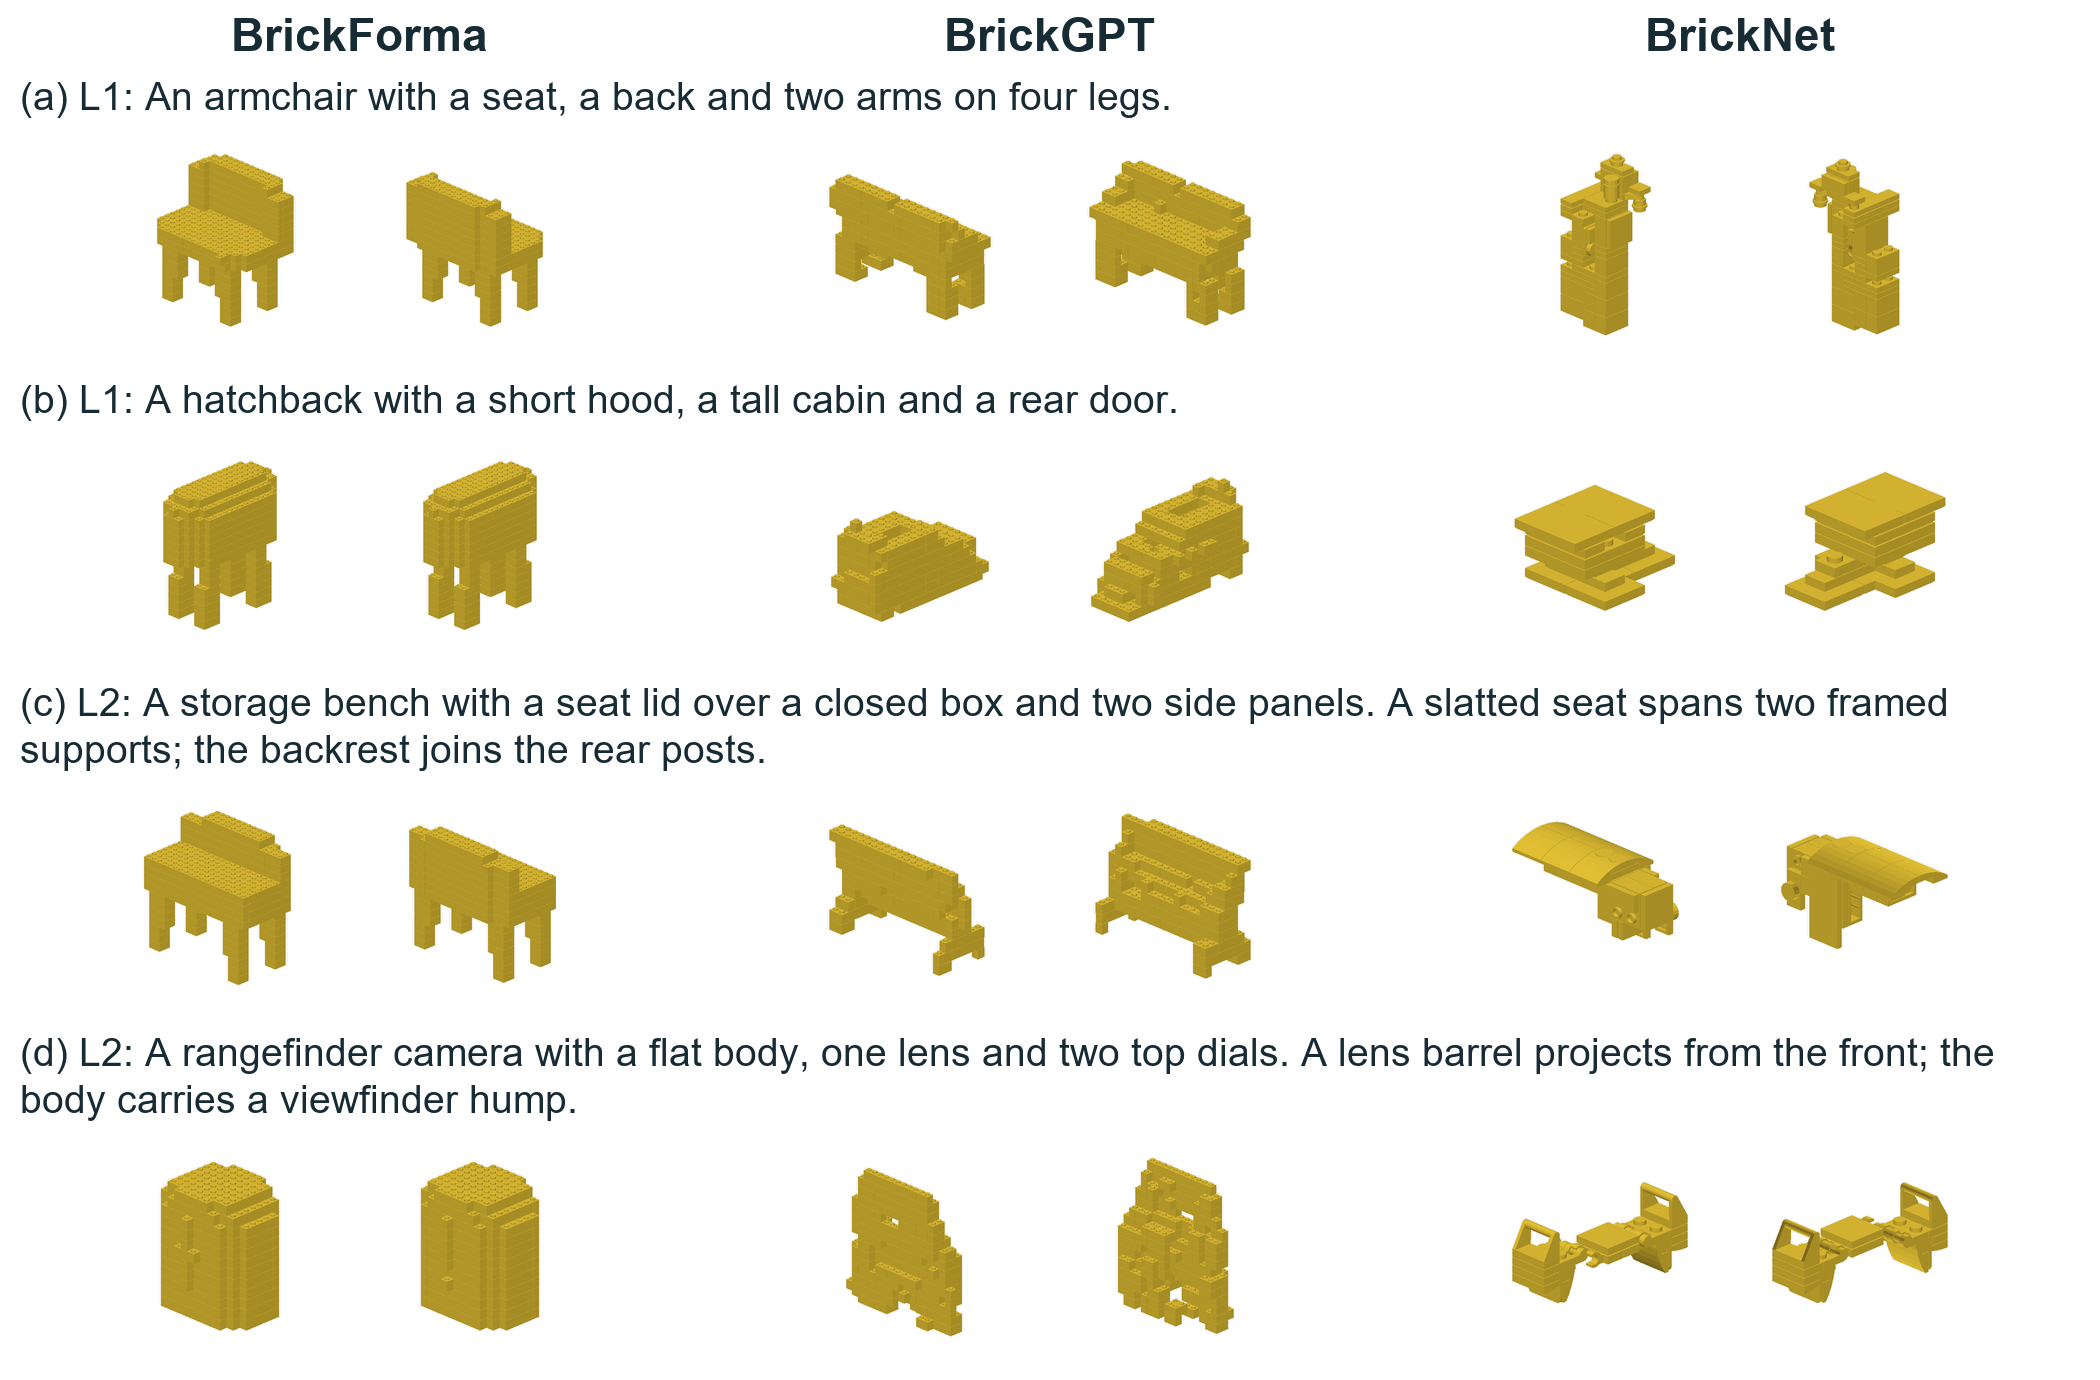
\includegraphics[width=\textwidth]{figures/matched_short_prompts_20261116.png}
\caption{Four examples from the matched evaluation with the same prompts, render settings, and azimuths ($45^\circ$ and $225^\circ$) across systems. The highest VQAScore belongs to BrickForma for the chair and bench, BrickGPT for the hatchback, and BrickNet for the camera.}
\label{fig:gallery}
\end{figure*}


% \subsection{Raw versus Refined Outputs}
% \begin{table}[t]
\centering
\small
\begin{tabular}{lrr}
\toprule
Metric & Raw & Refined \\
\midrule
$P_{\mathrm{inv}}$ $\downarrow$ & 0.1897\% & 0.0000\% \\
VQAScore $\uparrow$ & 0.2065 & 0.2071 \\
PE $\uparrow$ & 0.1858 & 0.1859 \\
SigLIP2 $\uparrow$ & 0.1379 & 0.1261 \\
Mean parts & 178.7 & 421.2 \\
\bottomrule
\end{tabular}
\caption{Earlier repair comparison on 110 pairs sharing the same prompt, model identifier, and caption.}
\label{tab:raw-refined}
\end{table}

% To quantify the impact of exact-cover reconstruction, we examine 110 raw/refined pairs from an earlier 114-prompt comparison sharing identical prompts and model identifiers (Table~\ref{tab:raw-refined}). Refinement eliminates invalid placements ($P_{\mathrm{inv}}$ drops from 0.1897\% to 0.0000\%) and increases mean part count from 178.7 to 421.2. VQAScore and PE remain essentially unchanged, whereas SigLIP2 shifts from 0.1379 to 0.1261.

\subsection{Geometric Refinement Audit}
\label{sec:diagnostics}
Defining stud contacts by footprint overlap across adjacent layers, we map the same 110 pairs onto a grid with 20 LDU horizontal pitch and 24 LDU layer height and align each export to a common occupied-cell origin. All 110 pairs preserve identical occupied voxel unions after translation, while single-component assemblies rise from 18 to 110 and overlap-free layouts rise from 100 to 110 (Table~\ref{tab:export-audit}).
\begin{table}[t]
\centering\small
\begin{tabular}{@{}lrr@{}}
\toprule
Export measure & Raw & Refined \\
\midrule
Single stud component & 18/110 & 110/110 \\
Mean stud components & 4.29 & 1.00 \\
No body-cell overlap & 100/110 & 110/110 \\
\midrule
\multicolumn{3}{@{}l@{}}{Equal voxel unions after translation: 110/110} \\
\bottomrule
\end{tabular}
\caption{Earlier export audit of 110 matched raw/refined pairs. Union equality uses translation normalization.}
\label{tab:export-audit}
\end{table}


In the separate 525-prompt diagnostic run, only 46 raw drafts form a single stud component, whereas all 525 final layouts achieve single-component connectivity while preserving their target voxel unions after the recovery procedure (Appendix~\ref{app:eval}).

\subsection{Evaluation Boundaries}
Our benchmark compares delivered exports from systems that differ in inference settings and part libraries, while description levels vary in both semantic detail and token length---truncating 121 prompts in PE and 209 in SigLIP2 (Appendix~\ref{app:eval}). Uniform yellow rendering isolates geometric form and layout without assessing color fidelity, and the paired refinement audit covers delivered pairs, excluding unsuccessful solver attempts from its denominator.

\section{Limitations and Discussion}
Our experiments evaluate the combined data-construction and fine-tuning pipeline; isolating the specific contribution of LLM-authored generators relative to hand-crafted procedural baselines under a matched training budget remains future work. Moreover, while dataset release checks verify grounding and coverage and inference refinement enforces a single stud-connected component, physical stability and feasible assembly ordering require dedicated structural measurements. Finally, the integrated dataset release and the fine-tuning run record their sample counts separately (Table~\ref{tab:training-data}).

\section{Conclusion}
BrickForma crystallizes LLM-authored parametric programs into checked voxel-to-brick targets to fine-tune Qwen3-1.7B for \texttt{Text-to-Brick} assembly. On 525 matched prompts spanning five description levels, its raw outputs lead all three text--image alignment metrics while keeping mean invalid placements at 0.79\%. Paired with exact-cover MILP refinement that enforces stud connectivity while preserving the voxel union, this division of labor offers a practical path toward constructive 3D spatial reasoning in compact models.

% Camera-ready only: uncomment for non-anonymous version.
% \section*{Author Contributions}
% H.L. and R.L. conceived the initial study design and formulated the research questions.
% Z.X. designed and implemented the LLM-assisted parametric voxel generation pipeline (80,000 models and 400,000 L1--L5 descriptions) and developed the dataset-level voxel-to-brick conversion and local refinement algorithms.
% H.L. conducted the parameter-efficient LoRA fine-tuning of the Qwen3-1.7B backbone.
% Z.X. and H.L. co-developed the inference-time voxel-union and MILP exact-cover refinement pipeline, and E.W. formalized its algorithmic specification and pseudocode (Algorithm~\ref{alg:inference-refinement}).
% R.L. established the standardized multi-view evaluation protocol, implemented the alignment and validity metrics, and designed the figures and tables.
% R.L. and Z.X. executed the BrickForma inference runs and wrote the manuscript.
% H.L., R.L., Z.X., E.W., and S.W. conducted the large-scale benchmark evaluations across the BrickGPT, BrickNet, and untuned Qwen3-1.7B baselines.
% % X.Q. supervised the project and revised the manuscript.
% All authors discussed the results and approved the final manuscript.
\bibliography{references}
\FloatBarrier
\appendix
\section{Technical Appendix: Dataset Details}
\label{app:dataset}
The historical figures and tables in this appendix retain the supplied measurements and model renders, with labels translated into English. They use release-specific versions and criteria and are not substitutes for the integrated statistics or the current main comparison.

\paragraph{Contact-based gravity screening.}
We model 8\,mm stud spacing, 9.6\,mm brick height, and 1\,g per occupied stud-brick cell. Each overlapping stud contributes four vertical contact points at the corners of a square with half-width 0.25 stud. The horizontal ground can only provide compression at the corners of ground-level brick footprints inset by 0.05 stud. A linear program (LP) seeks vertical force balance and balance of the two gravity-induced moments for every brick. We verify the resulting contact forces against these equations. After the final assembly passes, the same check is applied to the bricks through each completed layer, bottom to top. Each stud-connected component of a prefix is checked independently on the unanchored ground.

\paragraph{Tipping margin and clutch demand.}
The tipping margin is the minimum signed inward distance from the horizontal center-of-mass projection to the edges of the convex hull of the ground contacts. We convert the margin from studs to meters and reject zero or negative margins within numerical tolerance. If the compression-only LP is infeasible after this check, a second LP permits tension at internal stud contacts. It minimizes the largest total tensile force across the four contact points of any single stud. We report this minimum required clutch force in newtons per stud. Actual clutch capacity is uncalibrated. A verified compression-only solution qualifies for a gravity-screening pass, while solutions requiring tensile support are recorded separately.

\emph{Caption example.} The five captions of one model share a prefix and add detail level by level. The L1 prompt is \textquotedblleft An oval birdhouse with curved roof, enclosed room and front entrance.\textquotedblright\ Its L5 description is: ``An oval birdhouse with curved roof, enclosed room and front entrance. The protective roof joins the walls; the circular front entrance reaches a real interior cavity. Curved substantial surfaces carry their continuously attached functional parts. Overall width is 1.15 times depth; height is 0.80 times width. Parts follow functional positions. Continuous red, tan, brown color regions distinguish the body and attachments. The front reveals functional parts; side and top views reveal depth, connections and layout.''

\begin{table}[!htbp]
\centering
\small
\setlength{\tabcolsep}{3pt}
\begin{tabular}{lrrr}
\toprule
Release & Passing & Added & Removed \\
\midrule
Strict v3 & 7,902 & -- & -- \\
Relaxed & 65,503 & 428,278 & 38,230 \\
Local refinement & 79,298 & 228,582 & 125 \\
\bottomrule
\end{tabular}
\caption{Geometric pass counts of the 80,000 source models under successive conversion releases (relaxed: several grounded components allowed), with total voxels added and removed, as in the corresponding release reports.}
\label{tab:conversion}
\end{table}

\begin{figure*}[!htbp]
\centering
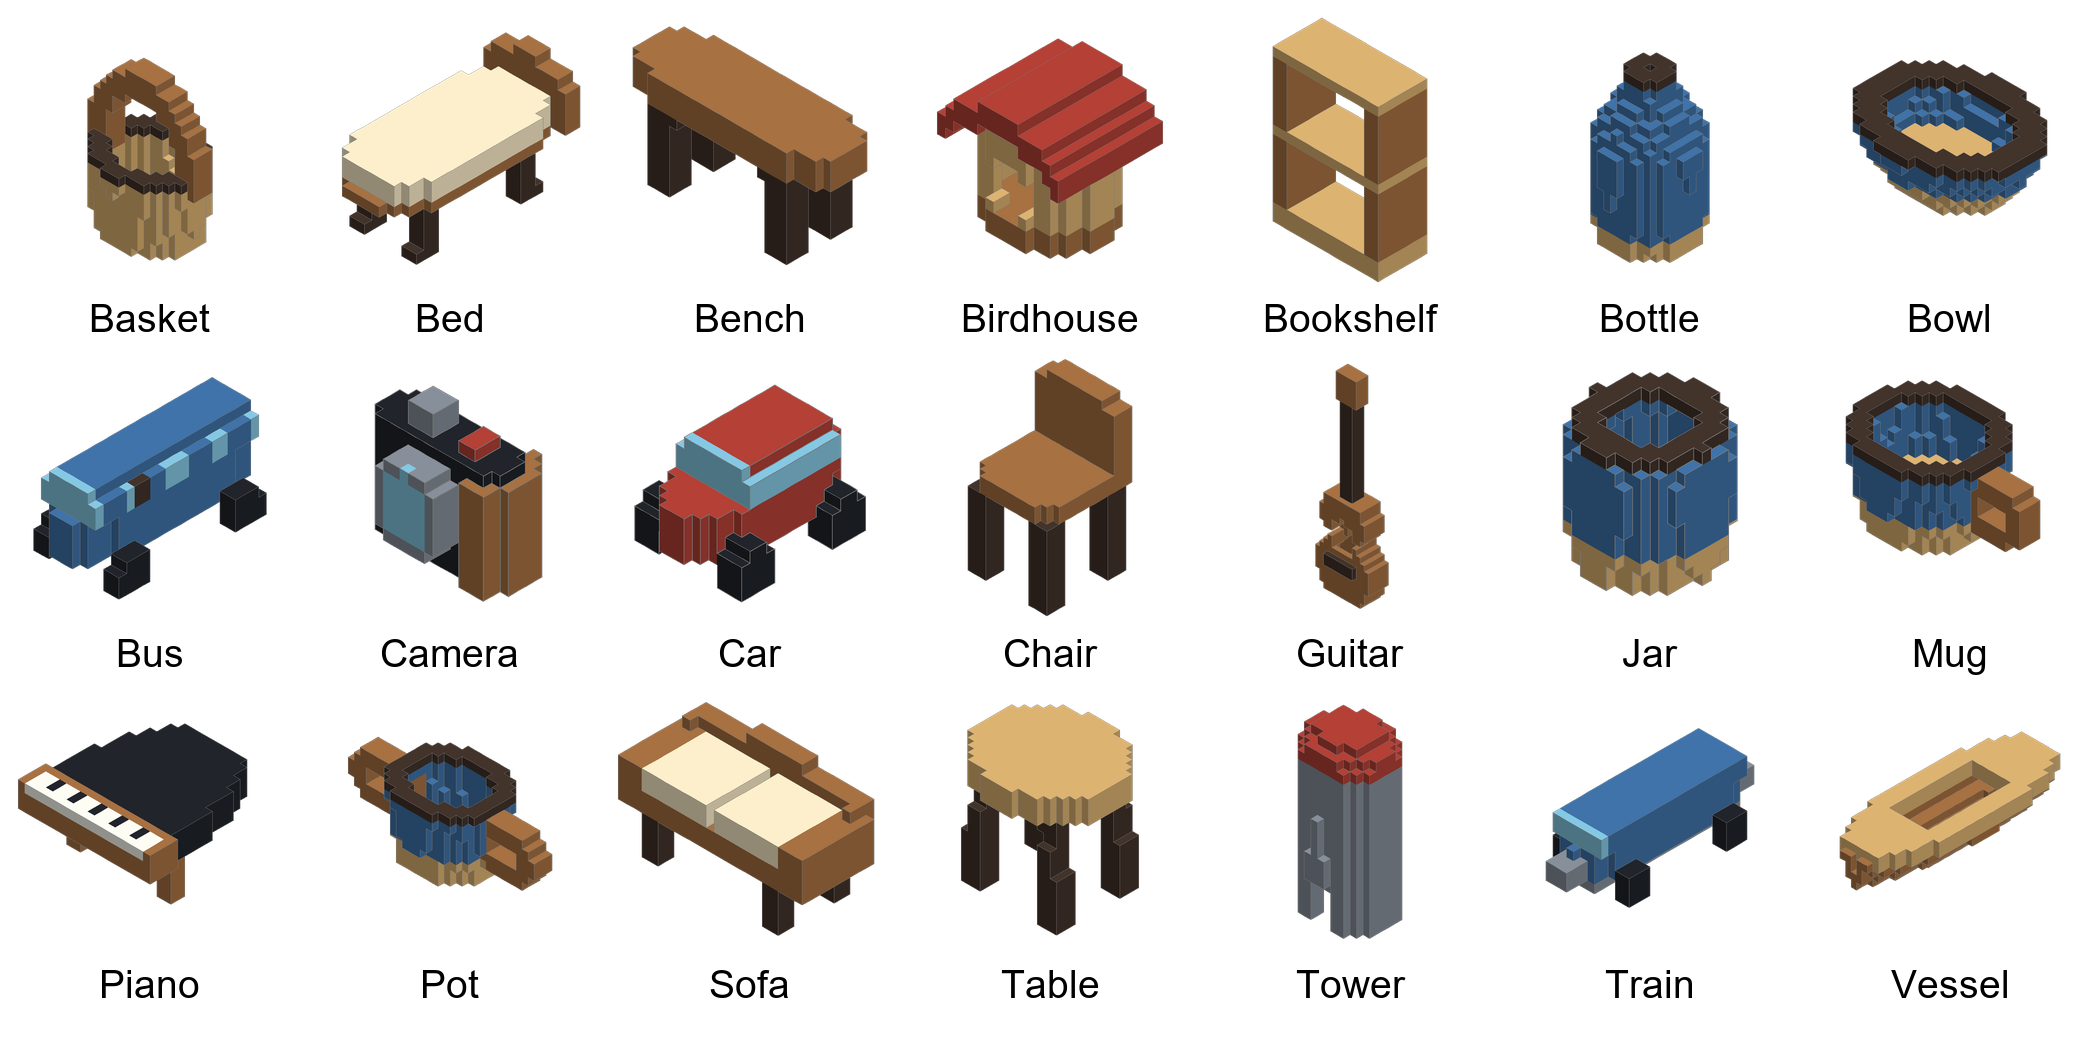
\includegraphics[width=\textwidth]{figures/image7_en.png}
\caption{Voxel model samples spanning the 21 object categories.}
\end{figure*}

\begin{figure*}[t]
\centering
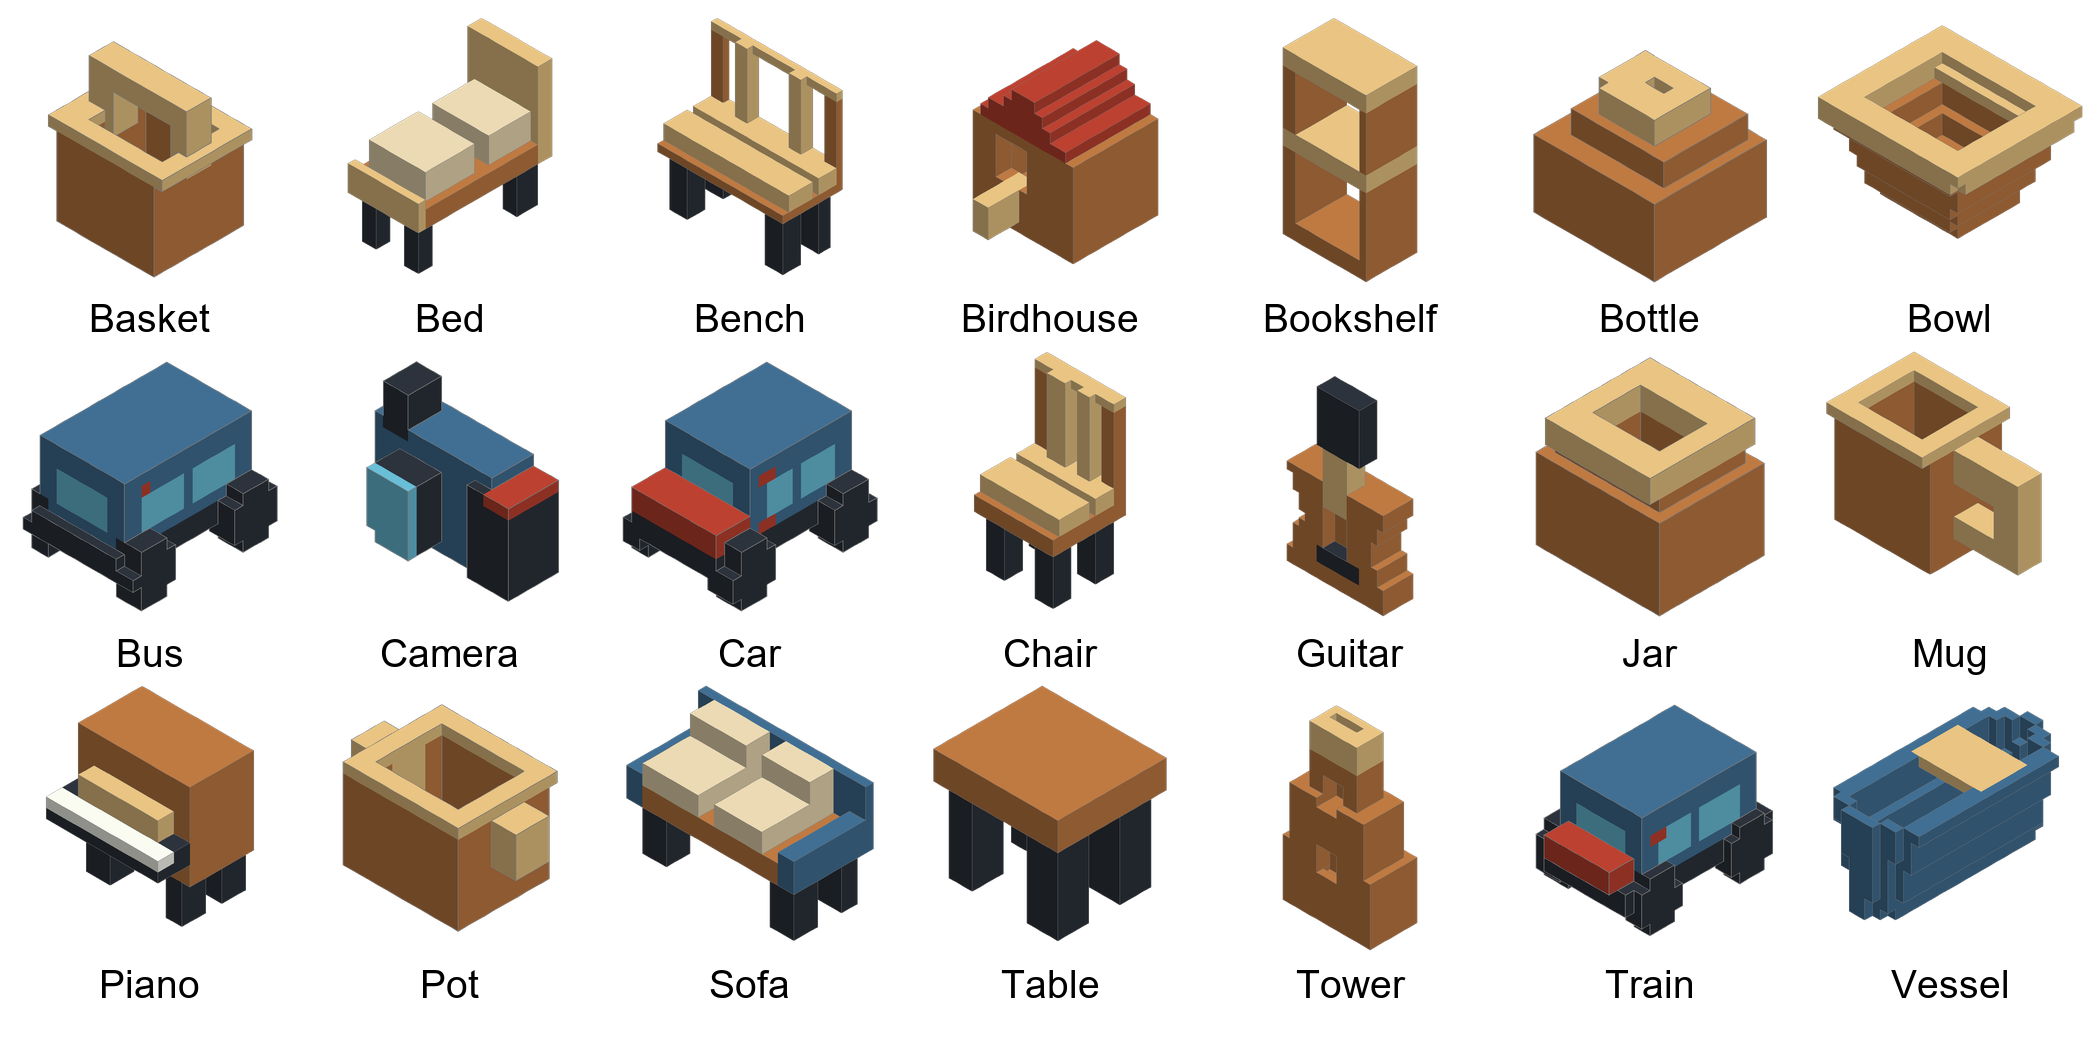
\includegraphics[width=\textwidth]{figures/image8_en.png}
\caption{Additional historical voxel model examples.}
\end{figure*}

\begin{figure*}[!htbp]
\centering
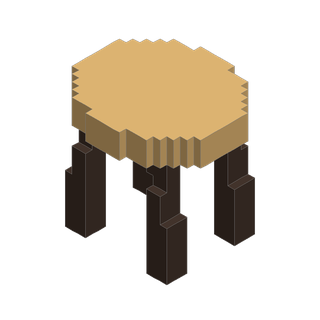
\includegraphics[width=0.118\textwidth]{figures/image4.png}\hfill
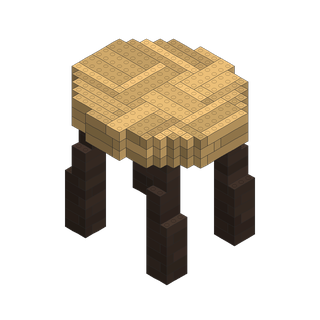
\includegraphics[width=0.118\textwidth]{figures/image5.png}\hfill
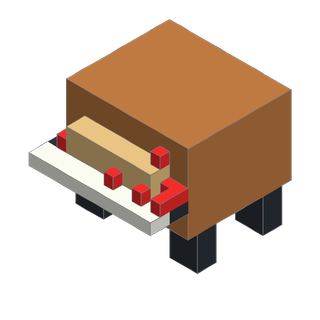
\includegraphics[width=0.118\textwidth]{figures/image2.png}\hfill
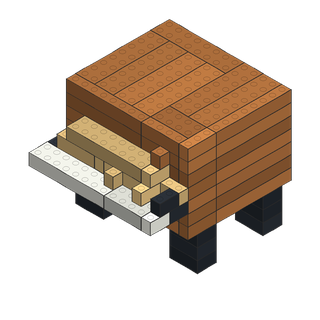
\includegraphics[width=0.118\textwidth]{figures/image3.png}\hfill
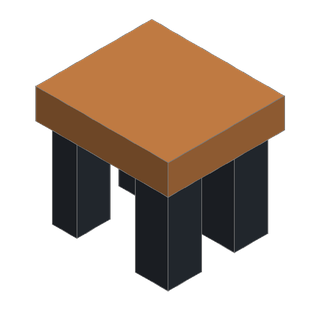
\includegraphics[width=0.118\textwidth]{figures/image9.png}\hfill
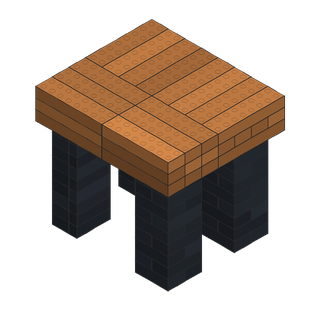
\includegraphics[width=0.118\textwidth]{figures/image10.png}\hfill

\includegraphics[width=0.118\textwidth]{figures/image11.png}\hfill
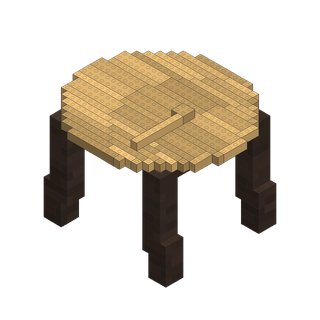
\includegraphics[width=0.118\textwidth]{figures/image12.png}
\caption{Historical examples of voxel targets and brick layouts after local repair.}
\end{figure*}

\begin{figure*}[t]
\centering
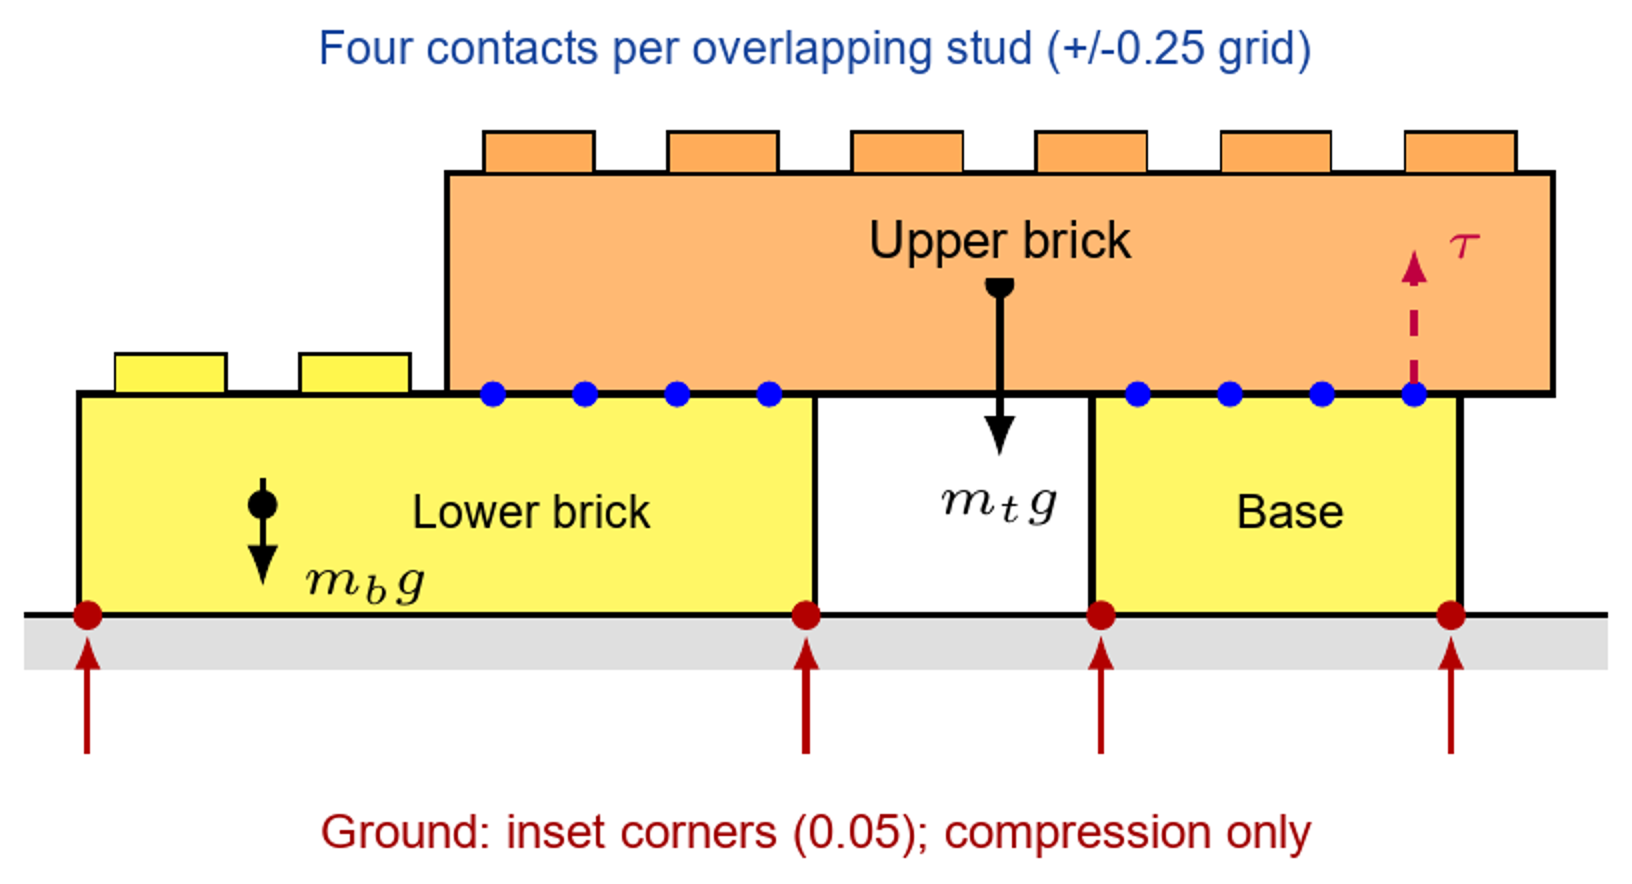
\includegraphics[width=0.75\textwidth]{figures/image13_en.png}
\caption{Historical contact-based gravity screening model, with English labels. The stated contact and ground assumptions are retained.}
\end{figure*}

\begin{figure*}[!htbp]
\centering
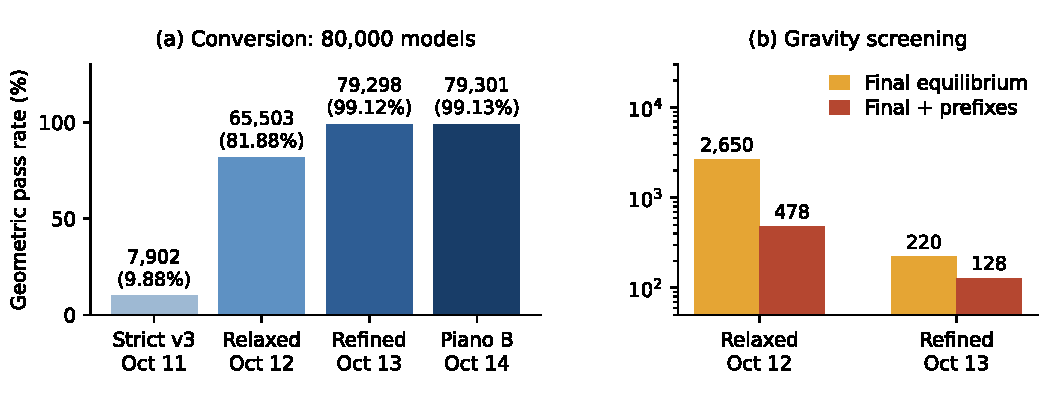
\includegraphics[width=\textwidth]{figures/image14_en.pdf}
\caption{Historical comparison of geometric conversion and screening outcomes across releases; values as in the corresponding release reports (Table~\ref{tab:conversion}).}
\end{figure*}

\begin{figure*}[!htbp]
\centering
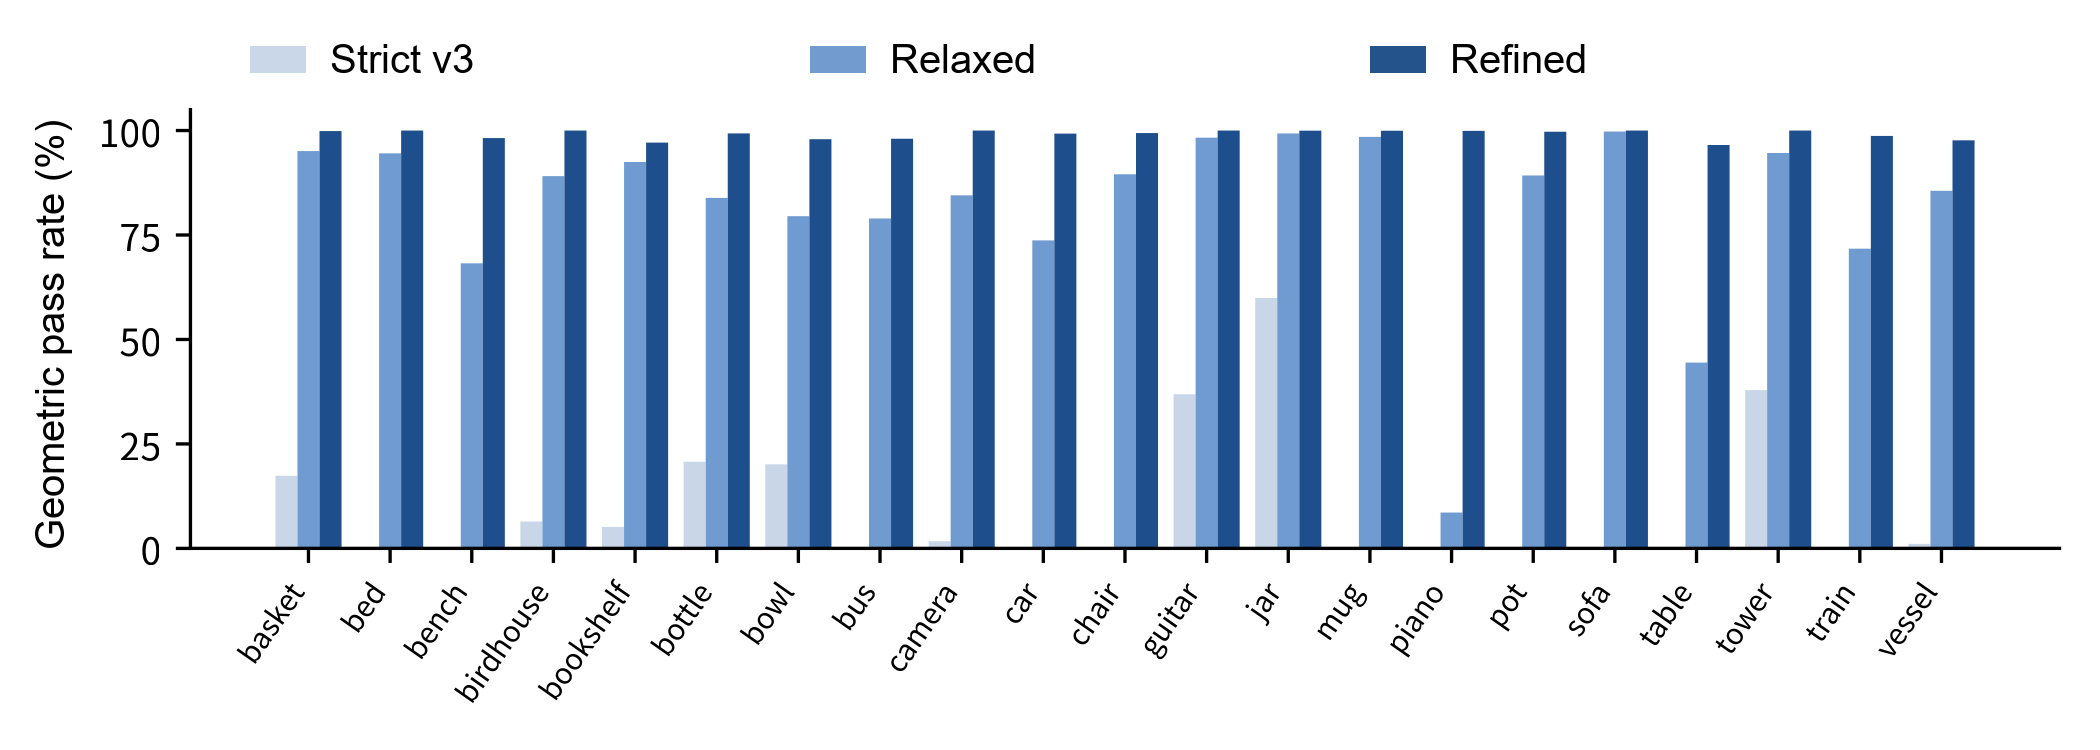
\includegraphics[width=\textwidth]{figures/image15_en.png}
\caption{Geometric pass rates by category for the three conversion releases in Table~\ref{tab:conversion}.}
\end{figure*}

\begin{figure*}[t]
\centering
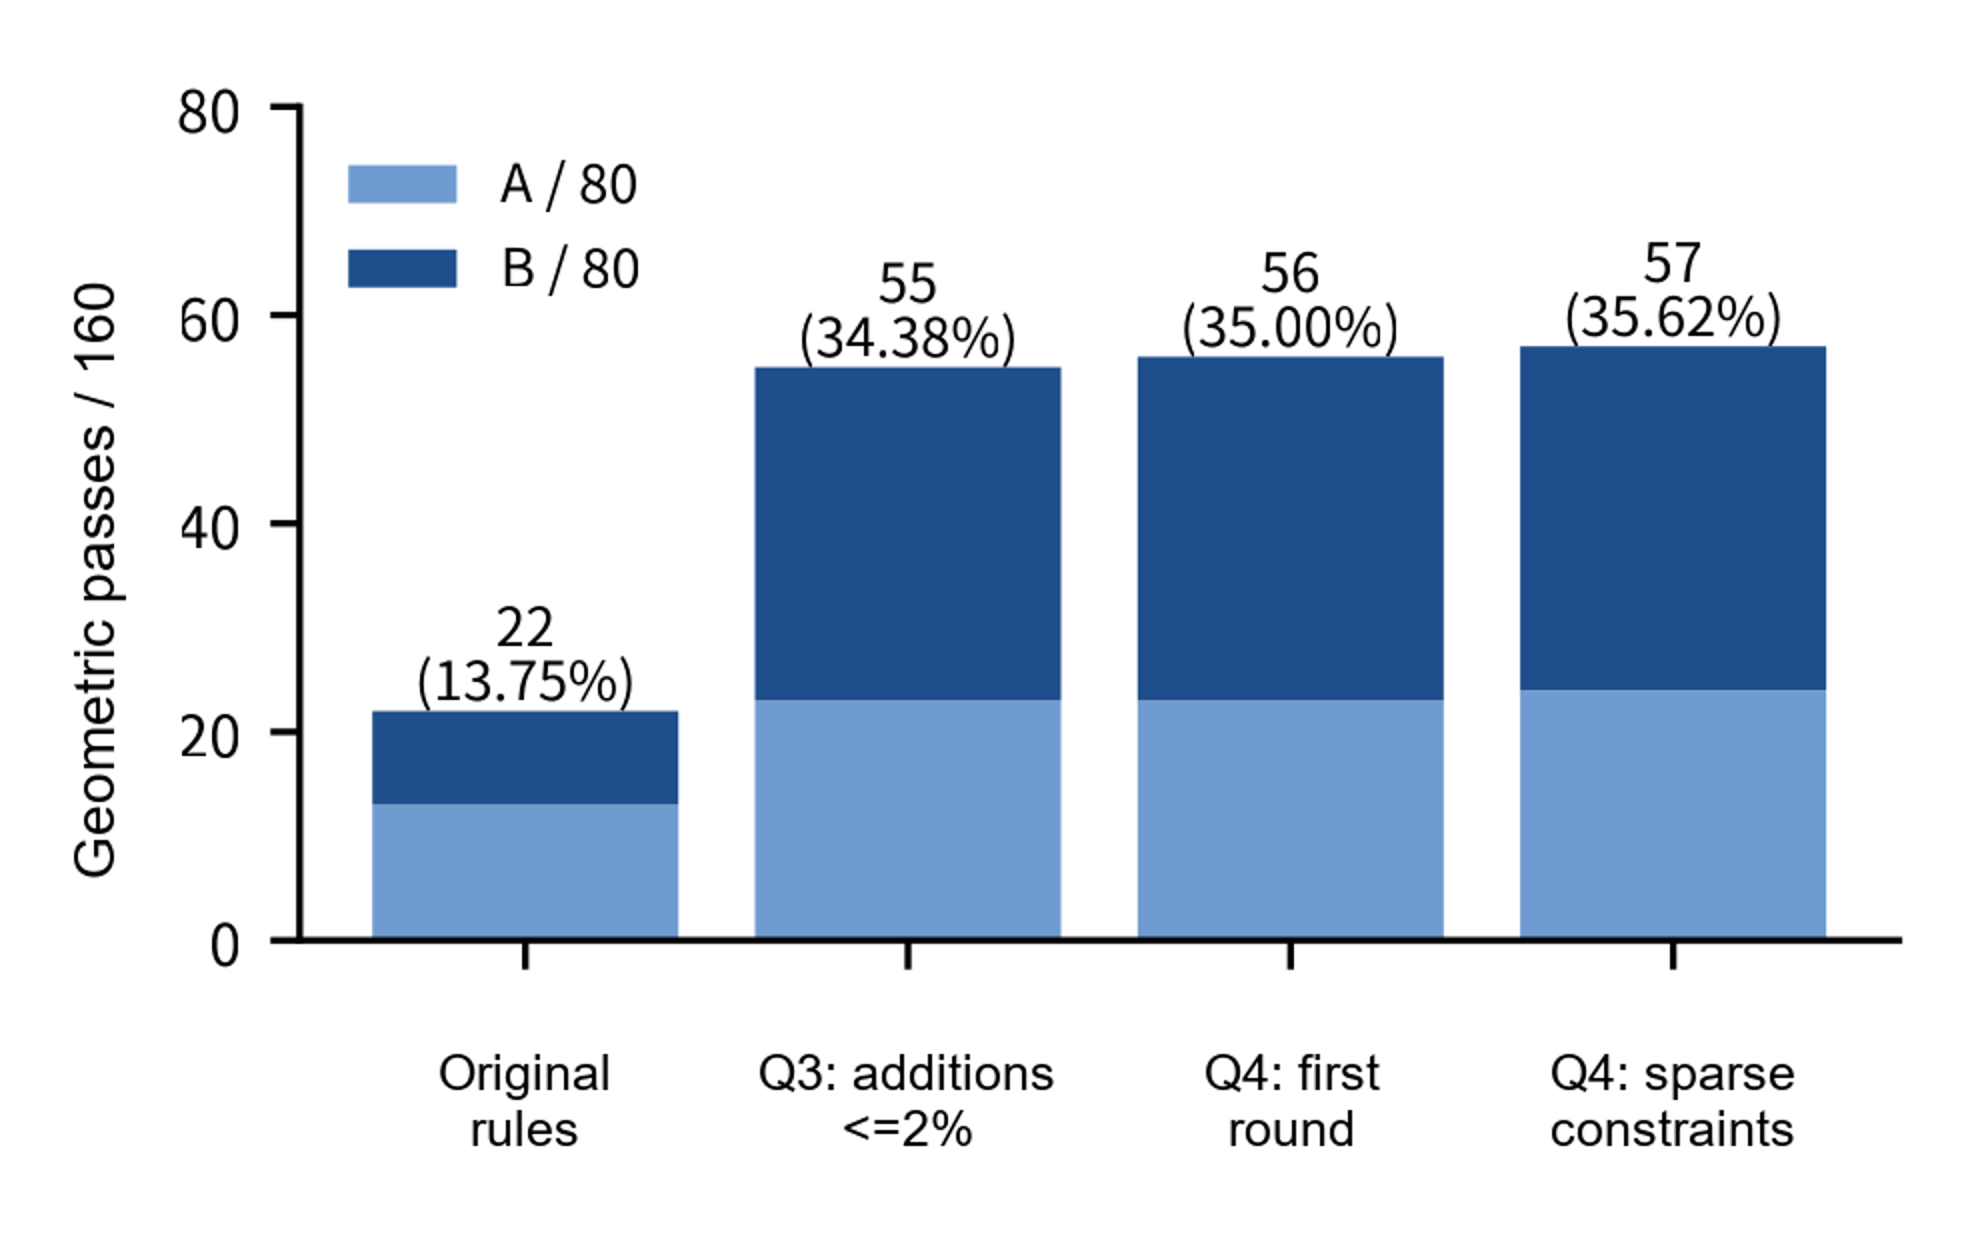
\includegraphics[width=0.72\textwidth]{figures/image16_en.png}
\caption{Geometric pass counts for the original rules, Q3, and two Q4 variants on the same 160-model sample (seed 38177). The Q4 rounds reuse this sample for tuning.}
\end{figure*}

\begin{figure*}[!htbp]
\centering
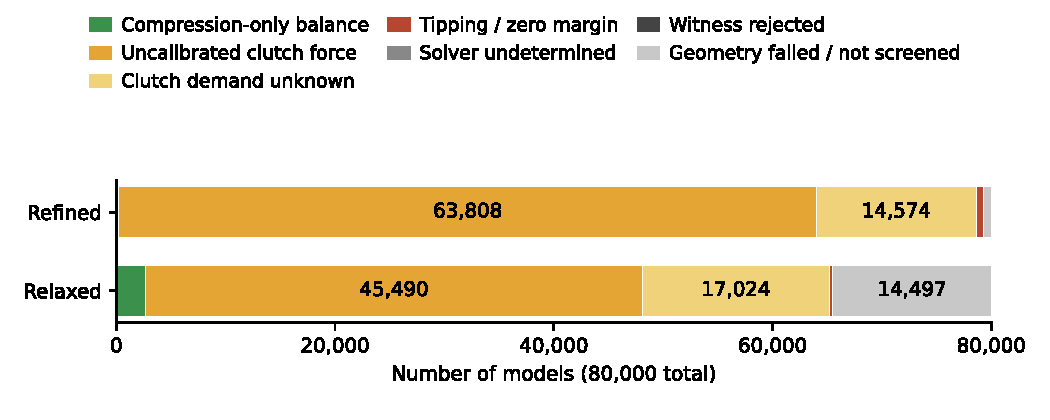
\includegraphics[width=\textwidth]{figures/image17_en.pdf}
\caption{Historical distributions of physical screening statuses; values as in the corresponding release reports. Counts refer to the specific releases shown and are kept separate from geometric pass rates.}
\end{figure*}


\section{Technical Appendix: Training Details}
\label{app:training}
Aggregate throughput is 24,448 tokens/s over eight GPUs, and the mean training loss is 0.0273. Evaluation and checkpointing run every 500 steps. With TRL~0.15, the unpacked multi-GPU path hangs after the first backward pass, which is why the TRL~0.17 stack is pinned. Because validation loss is lowest during epoch 2, two epochs would be a more economical setting for future runs (about one third less compute). The full software stack is transformers 4.51.3, trl 0.17.0, peft 0.15.2, datasets 3.6.0, and accelerate 1.6.0, with bf16 precision, gradient checkpointing, and unpacked sequences.

\begin{table}[!htbp]
\centering
\small
\begin{tabular}{lrr}
\toprule
Progress & Step & Validation loss \\
\midrule
Start & 500 & 0.1410 \\
--- & 1,500 & 0.0950 \\
--- & 10,500 & 0.0509 \\
--- & 22,500 & 0.0404 \\
$\approx$ End of epoch 1 & 44,500 & 0.0337 \\
--- & 65,500 & 0.0316 \\
Best (epoch 1.77) & 79,000 & 0.0308 \\
End of epoch 3 & 133,860 & 0.0339 \\
\bottomrule
\end{tabular}
\caption{Validation loss on the 2,000-sample validation subset. One epoch is $\approx$44,620 steps; the nearest evaluation to the end of epoch 1 is step 44,500.}
\label{tab:eval-loss}
\end{table}

% BrickGPT-paper column verified against arXiv:2505.05469 (Sec. 5.1 and Appendix A training details).
\begin{table*}[!htbp]
\centering
\small
\setlength{\tabcolsep}{5pt}
\begin{tabular}{lcc}
\toprule
Dimension & BrickGPT paper & Official Qwen3 script (ours) \\
\midrule
Base model & LLaMA-3.2-1B-Instruct & Qwen3-1.7B \\
LoRA & $r=32$, $\alpha=16$, dropout $0.05$, $q$/$v$ only (3.4M params) & $r=16$, $\alpha=32$, all linear layers \\
Learning rate & $2{\times}10^{-3}$ (AdamW) & $10^{-4}$ \\
Effective batch & 64 & 8 \\
Max length & 4,096 & 8,192 \\
Epochs & 3 & 3 \\
Hardware & 8$\times$RTX A6000, 12\,h & 8$\times$4090D, 25.3\,h \\
Data & StableText2Brick, 47k structures / 240k prompts & BrickForma-48, 79.3k models / 396,610 samples \\
\bottomrule
\end{tabular}
\caption{Our configuration versus the original BrickGPT paper \cite{brickgpt}. BrickGPT-paper values are taken from Sec.~5.1 and Appendix~A of arXiv:2505.05469 (base model, LoRA $r{=}32$, $\alpha{=}16$, dropout $0.05$, $q$/$v$ only with 3.4M parameters, AdamW learning rate $0.002$, global batch 64, 4096-token length filter, 3 epochs, 8$\times$RTX A6000 and 12\,h, and 47k+ structures / 240k prompts). The data organization, instruction template, absence of thinking mode, and LoRA paradigm follow BrickGPT; concrete hyperparameters follow the official Qwen3 adaptation, with the budget adjusted for the larger world, library, and corpus.}
\label{tab:brickgpt-recipe}
\end{table*}


\section{Technical Appendix: Additional Evaluation Material}
\label{app:eval}

\paragraph{Matched evaluation.}

The 525 matched prompts combine 265 previously delivered BrickForma Q8\_0 exports with 260 supplemental exports. We score the single raw export supplied for each prompt. This protocol measures the delivered drafts without filtering on completion or geometry, rerunning Algorithm~\ref{alg:inference-refinement}, or choosing a candidate by its scores. The supplemental records flag 8 incomplete generations and 96 failures of the source geometry check out of 260, with potential overlap. The 265 earlier exports lack corresponding completion and geometry flags. We score all 1,575 LDraw exports on all four metrics, using 12,600 rendered views for alignment. Three supplied GLB previews contain only a prefix, so we render from the delivered LDraw sequences in all cases. BrickGPT uses a $20^3$ world and seed 42, with recorded regeneration budgets of 8 or 100. For the 260 supplemental BrickForma exports, inference ran locally without MILP refinement using checkpoint \texttt{BrickGPT-Qwen3-1.7B-BrickMore-48} (revision \texttt{92d1c595}) in \texttt{bfloat16} precision with \texttt{sdpa} attention, \texttt{max\_new\_tokens}=8192, \texttt{temperature}=0.7, \texttt{top\_p}=0.9, and seed schedule $(42,104,2026)$, with zero overlap against the training set. The 265 earlier Q8\_0 exports come from an earlier inference batch whose per-sample decoding flags were not logged, and the 105-sample offset between $79{,}301{\times}5=396{,}505$ and the logged 396,610 training pairs stems from a minor snapshot offset between the final dataset release and the training run.

\begin{samepage}
\paragraph{Baseline versions.} The archived 260-prompt BrickGPT runner is based on GitHub commit \texttt{9c53c7c} of \url{https://github.com/AvaLovelace1/BrickGPT}. The generation report records a local checkpoint combining \texttt{meta-llama/Llama-3.2-1B-Instruct} and the public \texttt{AvaLovelace/BrickGPT} LoRA adapter. The runner can load a premerged checkpoint or merge those weights through PEFT's \texttt{merge\_and\_unload}. The report identifies the merged checkpoint used, with no separate merge log. The BrickNet GitHub reference snapshot is commit \texttt{283faf7} of \url{https://github.com/kulits/BrickNet}. The public 1.7B PT and SFT adapter revisions are \texttt{0f75d5e5} and \texttt{3fe7f4c1}, respectively, on \texttt{Qwen/Qwen3-1.7B}. The 265 other BrickGPT exports and the BrickNet exports lack a recorded generation-code commit. Invalid-placement scoring uses the inset collision kernel from the pinned \texttt{bricknet==0.1.0} PyPI wheel.

\paragraph{Reference dataset snapshots.} BrickGPT uses StableText2Brick (public data upload \texttt{1dcf904} at \texttt{AvaLovelace/StableText2Brick}). BrickNet uses the gated PT, SFT, and validation splits described in \texttt{DATA.md} at GitHub commit \texttt{283faf7}. The release documentation identifies those splits by file name and gives no separate dataset revision.
\end{samepage}


\paragraph{Untuned Qwen3-1.7B.} None of the 260 untuned outputs passed the generation-time geometry check. The strict parser found no placements in 178 outputs, and two used an unsupported part type. We assign these 180 outputs zero for VQAScore, PE, and SigLIP2 and retain the measured scores for the 80 scorable partial layouts. All alignment means use the same 260 prompts. For the 80 pairs with scorable base layouts, the mean file-order invalid-placement ratios were 39.67\% for the untuned model and 1.01\% for raw BrickForma. The comparison uses common scoring across delivered generation runs that can differ in decoding.

\paragraph{Paired tests and truncation.}
Table~\ref{tab:sig} compares alignment scores on the 525 prompts. We use a two-sided exact sign test and a two-sided Wilcoxon signed-rank test with the normal approximation, excluding ties. Holm correction is applied separately to the six comparisons within each test. All adjusted $p$ values are below $2.0{\times}10^{-8}$. PE truncates 121 prompts and SigLIP2 truncates 209. On the untruncated subsets, BrickForma / BrickGPT / BrickNet score 0.1510 / 0.1408 / 0.1135 on PE (404 prompts) and 0.0340 / 0.0157 / 0.0009 on SigLIP2 (316 prompts).

%Figure 9 and the related description
%\begin{table}[t]
\centering\small
\setlength{\tabcolsep}{3pt}
\begin{tabular}{llrrr}
\toprule
Baseline & Metric & W/L/T & Sign $p_H$ & Wilc.\ $p_H$ \\
\midrule
BrickGPT & VQAScore & 384/141/0 & $1.5\times 10^{-26}$ & $4.8\times 10^{-20}$ \\
 & PE & 337/188/0 & $1.6\times 10^{-10}$ & $3.1\times 10^{-12}$ \\
 & SigLIP2 & 327/198/0 & $2.0\times 10^{-8}$ & $7.3\times 10^{-12}$ \\
BrickNet & VQAScore & 460/65/0 & $1.6\times 10^{-73}$ & $4.6\times 10^{-60}$ \\
 & PE & 406/119/0 & $4.6\times 10^{-37}$ & $1.3\times 10^{-47}$ \\
 & SigLIP2 & 408/115/2 & $9.4\times 10^{-39}$ & $2.4\times 10^{-42}$ \\
\bottomrule
\end{tabular}
\caption{Two-sided paired tests on 525 prompts. W/L/T counts BrickForma wins, losses and ties. Each test uses Holm correction across six comparisons.}
\label{tab:sig}
\end{table}


%\paragraph{Earlier 114-prompt comparison.} BrickGPT outputs were generated in its native $20^3$ world (seed 42), whereas BrickForma places bricks in a $48^3$ workspace, which partly explains the difference in part counts.
%The systems differ in candidate selection, filtering, and post-processing.
%On the BrickForma side, 45 of the 114 comparison outputs, together with their prompts, were chosen by human review as the best of six candidate phrasings in a category--level group; a winner was available in 79 of 105 groups, and 45 of those winners entered this comparison.
%The remaining 69 outputs come from later fill-in, regeneration, colleague, and review rounds: 35 replaced a judged winner in 34 groups, and 34 filled 26 groups in which no candidate had been judged acceptable; together the 114 outputs cover all 105 groups.\footnote{The six candidates are the five new-batch phrasings and one first-batch phrasing documented in the evaluation-set README. Among the 69: \texttt{review\_59} 21, a colleague success set 16, second-round redo 12, third-round fill-in 7, colleague \texttt{nine\_ldr} 7, regeneration 5, and \texttt{car\_trials} 1, as recorded in the 11-07 delivery manifest. BrickGPT was then run once on each selected prompt (seed 42); BrickNet contributed one accepted sample per prompt (up to 30 attempts).}
%The 114 outcomes comprised 110 refined layouts and four raw layouts. The earlier BrickGPT records report an eight-regeneration budget and Gurobi disabled.

%\paragraph{Sensitivity of the earlier comparison.}
With equal weighting over the 105 category--level groups, BrickForma scores 0.2347 / 0.1840 / 0.1257 and BrickGPT scores 0.1511 / 0.1459 / 0.0318 on VQAScore / PE / SigLIP2. After excluding prompts truncated by each encoder, PE is 0.1821 versus 0.1445 on 89 prompts and SigLIP2 is 0.1088 versus 0.0301 on 85 prompts. The PE and SigLIP2 text encoders read at most 72 and 64 tokens, respectively.

\paragraph{Inference refinement.}
For the clipped voxel union $C$, let $\mathcal{B}(v)$ index candidate placements from the oriented footprint library that cover $v$ and stay entirely within $C$. With binary placement variables $x_b$, exact coverage requires $\sum_{b\in\mathcal{B}(v)}x_b=1$ for each $v\in C$. This preserves the union and excludes overlaps. To enforce a single stud-connected component, a standard single-commodity flow formulation routes flow from a virtual root $r$ through directed stud-contact edges $(b,b')\in\mathcal{E}$ across adjacent layers: grounded candidate placements $b\in\mathcal{B}_{\mathrm{gnd}}$ receive root inflow $f_{r,b}\ge 0$, internal edge flows satisfy $0\le f_{b,b'}\le M x_b$ and $0\le f_{b,b'}\le M x_{b'}$ (for capacity bound $M=|C|$), and flow conservation $\sum_{(u,b)\in\mathcal{E}\cup\{(r,b)\}} f_{u,b} - \sum_{(b,v)\in\mathcal{E}} f_{b,v} = x_b$ ensures every selected placement is connected to the root. SciPy's HiGHS MILP interface uses the time tiers in Algorithm~\ref{alg:inference-refinement}. A feasible cover must also pass the independent placement, coverage, and connectivity audit. The logged run summaries record the solver time tiers and independent audit outcomes, while per-run objective weights and gap tolerances were not retained. Contact-based self-weight screening uses a separate LP (Appendix~\ref{app:dataset}).

\paragraph{Diagnostic cohort.}
We evaluate stud connectivity before and after geometric refinement on a separate set of 525 BrickForma generations, covering 21 categories, five description levels, and five phrasings per category--level combination. Algorithm~\ref{alg:inference-refinement} specifies the default rules for selecting a raw draft and refining its layout. For 28 prompts, recovery sampled seeds outside $S$. For two additional prompts, the solver budget was extended to 600\,s.

Before refinement, 46 of 525 raw layouts (8.8\%) formed a single stud-connected component. The counts for L1--L5 were 13, 9, 9, 7, and 8, with no clear trend across levels. Connectivity varied by category, with 8 of 25 sofa layouts passing and none of the 25 basket or 25 camera layouts passing. The other 479 raw layouts had at least two stud-connected components, with a median of five and a maximum of 33. Of these 479 layouts, 50 contained duplicated voxels, including 41 with at most five duplicated voxels. Among the 2,240 detached fragments, 1,320 were airborne and 920 were grounded.

After the full refinement and recovery procedure, all 525 final layouts formed a single stud-connected component and preserved the in-bounds voxel union of their corresponding raw draft (Table~\ref{tab:diag}). This diagnostic measures stud connectivity and preservation of the voxel union. Prompt fidelity and spatial reasoning remain outside its scope.

% \begin{figure*}[t]
% \centering
% 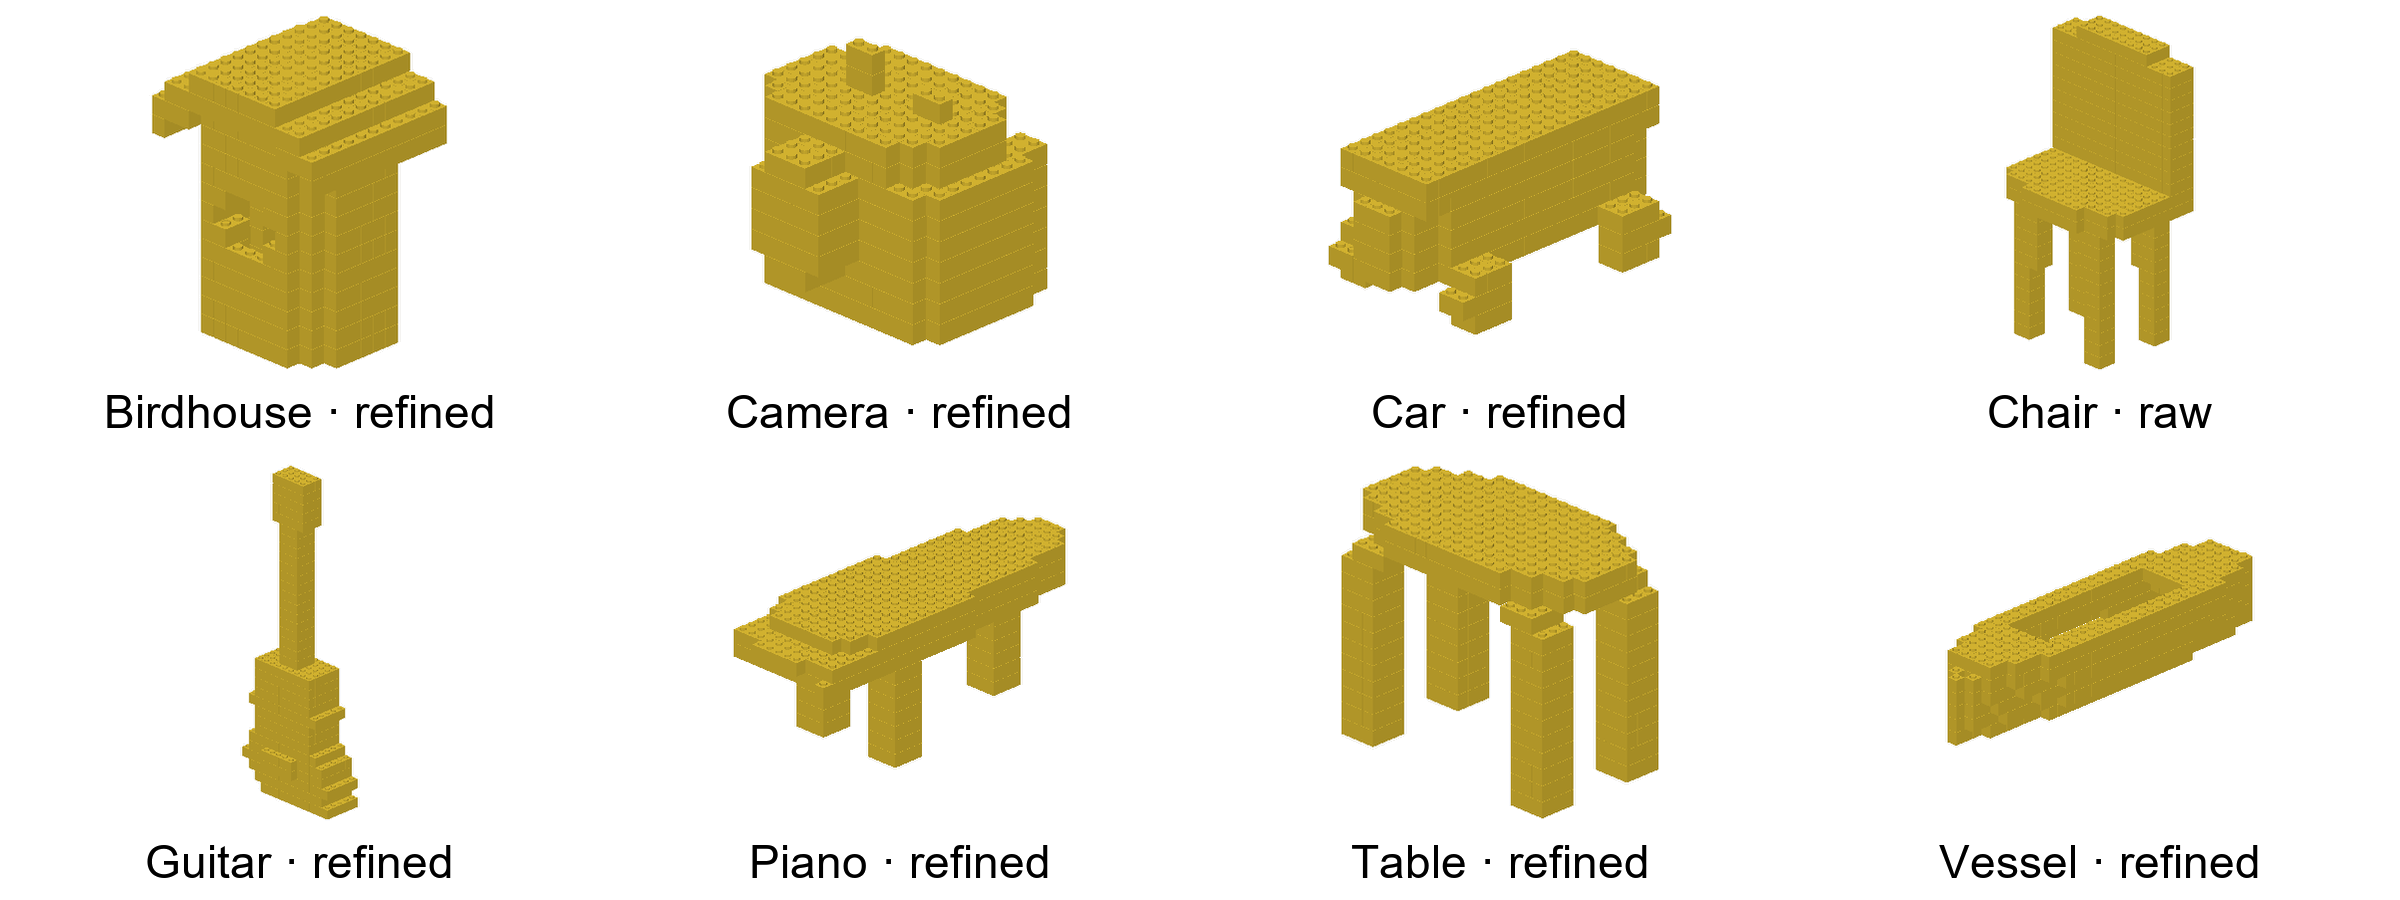
\includegraphics[width=\textwidth]{figures/generated_gallery_en.png}
% \caption{BrickForma outputs from the earlier 114-prompt comparison. The chair is raw and the remaining examples are refined.}
% \end{figure*}

\begin{table*}[!htbp]
\centering
\small
\setlength{\tabcolsep}{3pt}
\begin{tabular}{lr}
\toprule
Quantity (525 prompts) & Value \\
\midrule
Raw layout is a single stud component & 46 (8.8\%) \\
Stud components per failing raw (med./max) & 5 / 33 \\
Failing raw layouts with duplicated voxels & 50 / 479 \\
Detached fragments (airborne / grounded) & 1,320 / 920 \\
MILP tier reached (12 / 60 / 180 / 600\,s) & 326 / 133 / 18 / 2 \\
Prompts resampled outside $S$ & 28 \\
Final: single stud comp., union unchanged & 525 / 525 \\
Raw bricks, median (range) & 183 (77--623) \\
Final assembly bricks, median & 452 \\
\bottomrule
\end{tabular}
\caption{Structural diagnostics of raw outputs (Section~\ref{sec:diagnostics}). ``Union unchanged'' means the final assembly covers exactly the in-bounds voxel union of the raw draft; it does not assess whether the shape matches the prompt.}
\label{tab:diag}
\end{table*}



% \begin{figure*}[!htbp]
% \centering
% 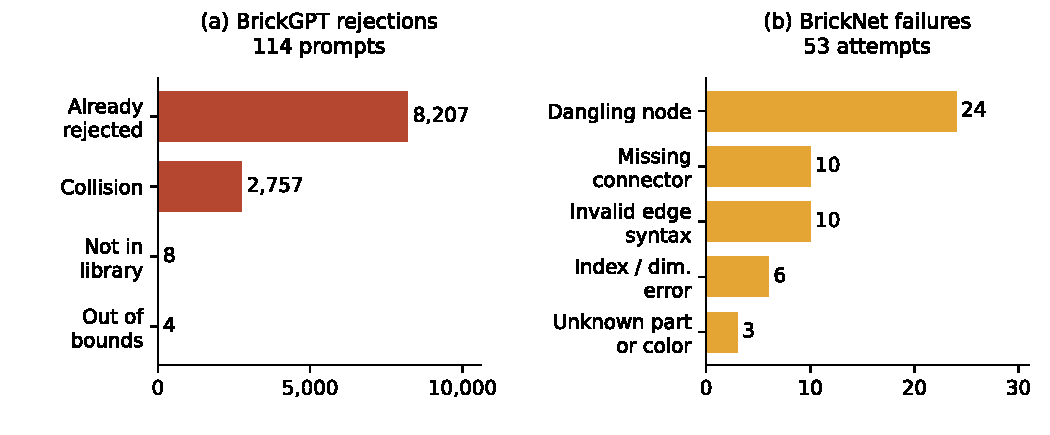
\includegraphics[width=\textwidth]{figures/image19_en.pdf}
% \caption{Historical failure categories in the supplied reference; values as in the corresponding run records.}
% \end{figure*}

\begin{figure*}[!htbp]
\centering
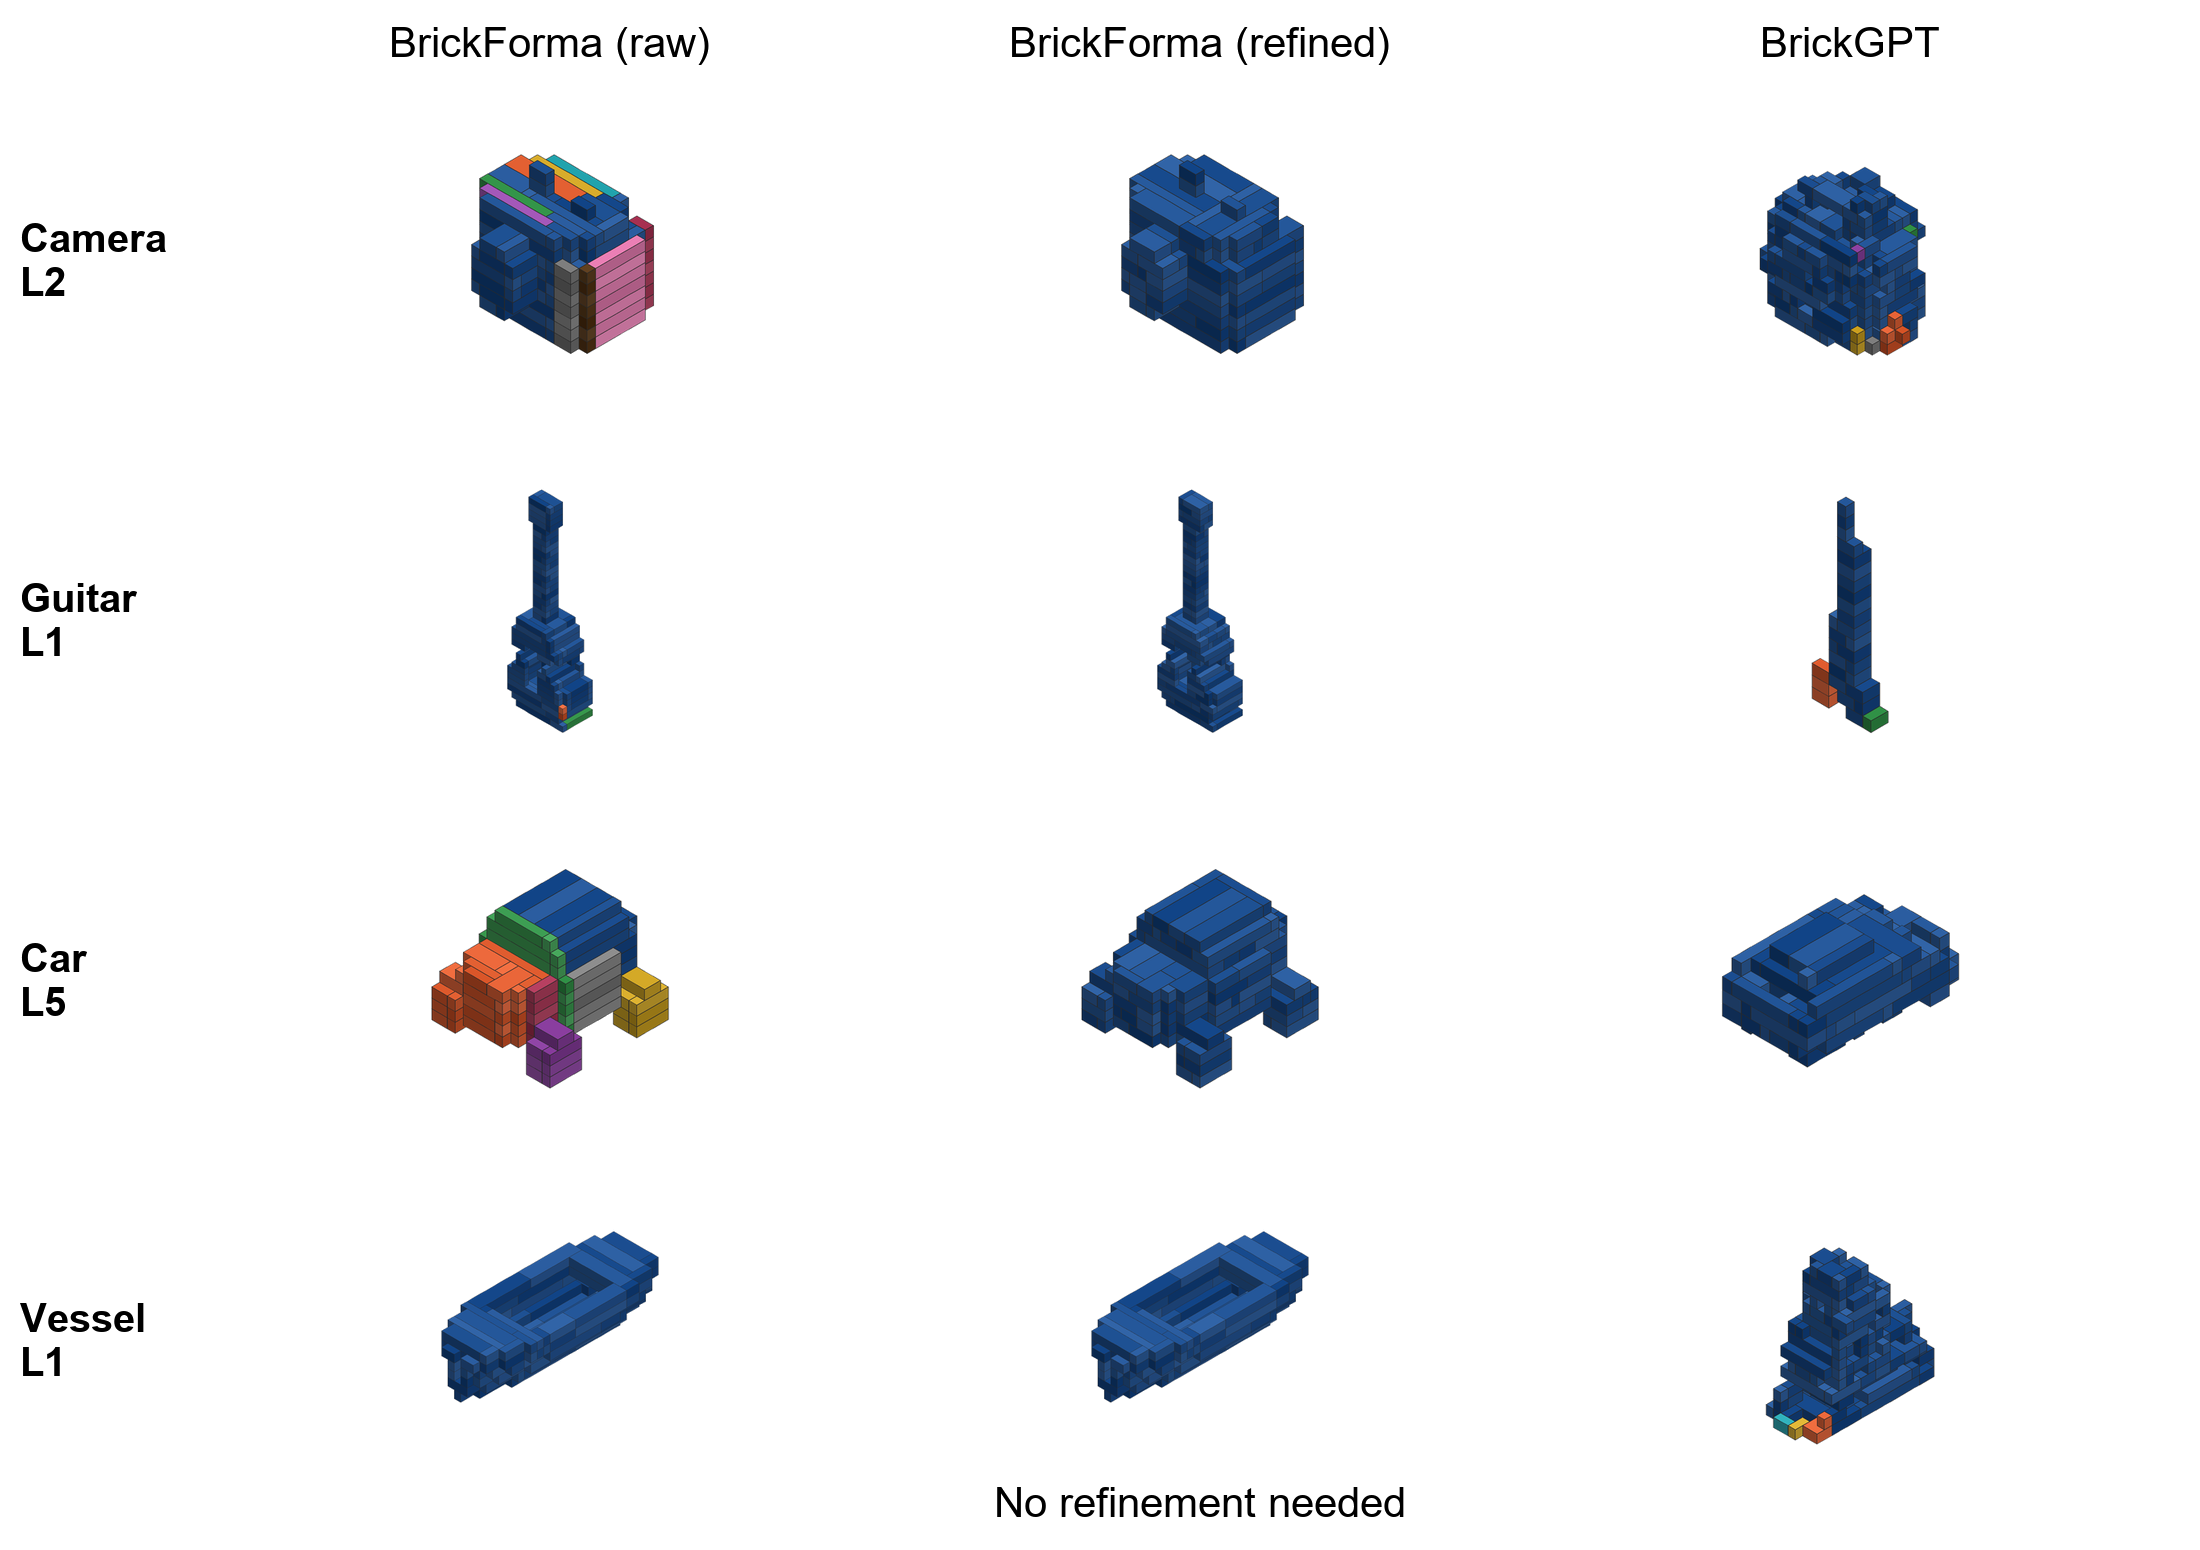
\includegraphics[width=\textwidth]{figures/original_comparison_en.png}
\caption{Qualitative historical examples from the supplied reference. Columns show raw and refined outputs of our system and BrickGPT outputs.}
\end{figure*}

\begin{figure*}[t]
\centering
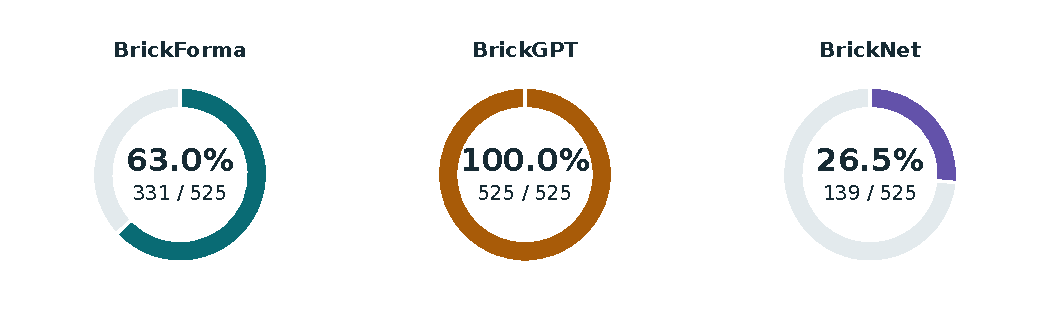
\includegraphics[width=\textwidth]{figures/comparison_20261117/01-zero-invalid.pdf}
\caption{Outputs with zero invalid placements on the 525 matched prompts. Colored arcs show $P_{\mathrm{inv}}=0$ and gray arcs show $P_{\mathrm{inv}}>0$. Each panel contains 525 outputs.}
\label{fig:comparison-zero-invalid}
\end{figure*}

\begin{figure*}[t]
\centering
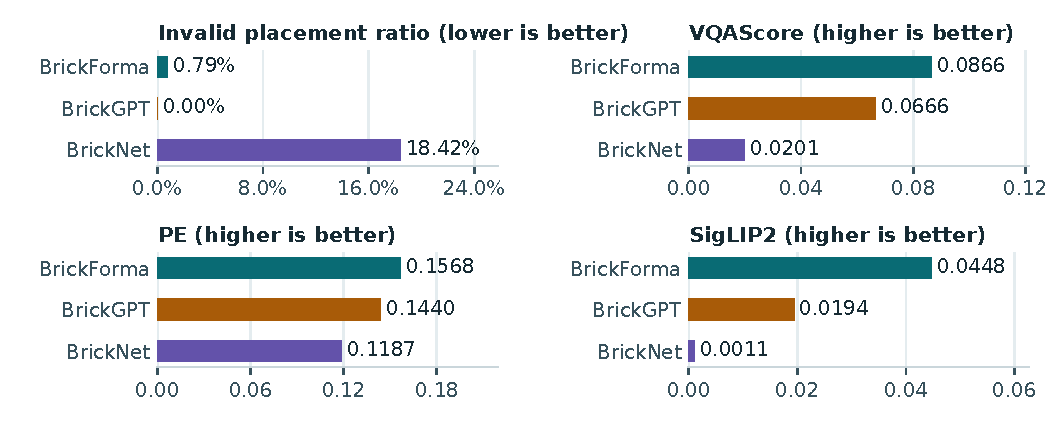
\includegraphics[width=\textwidth]{figures/comparison_20261117/02-means.pdf}
\caption{Mean scores on the 525 matched prompts. Each mean assigns equal weight to each prompt. The plotted values correspond to Table~\ref{tab:main}.}
\label{fig:comparison-means}
\end{figure*}

\begin{figure*}[t]
\centering
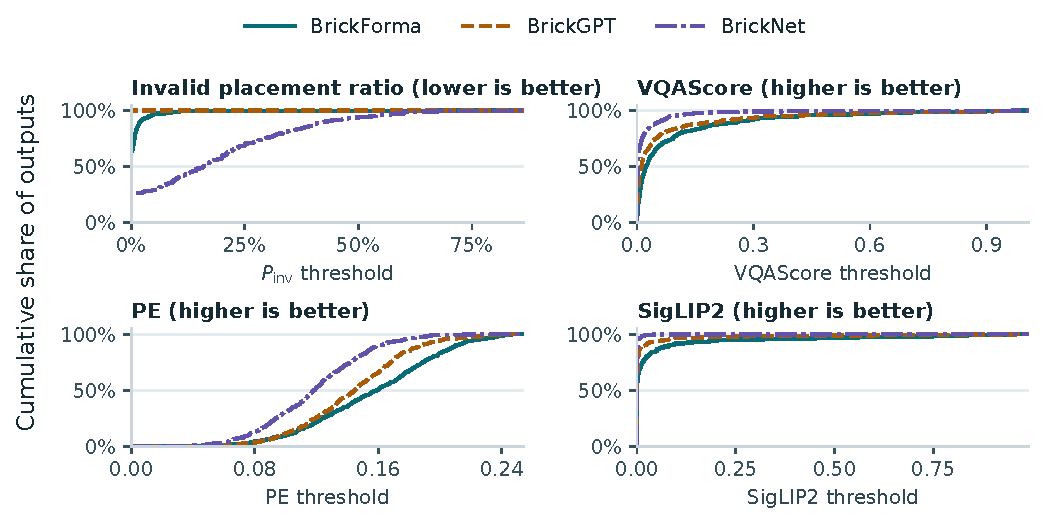
\includegraphics[width=\textwidth]{figures/comparison_20261117/03-distributions.pdf}
\caption{Empirical cumulative distributions of the four scores. Each curve gives the fraction of a system's 525 outputs at or below the threshold on the horizontal axis.}
\label{fig:comparison-distributions}
\end{figure*}

\begin{figure*}[t]
\centering
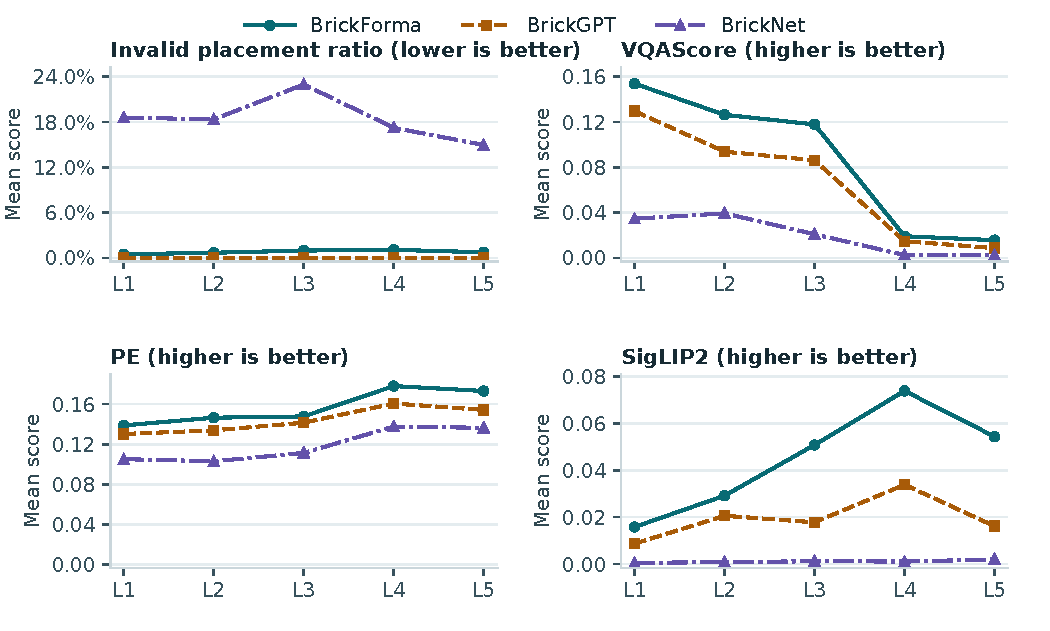
\includegraphics[width=\textwidth]{figures/comparison_20261117/04-by-level.pdf}
\caption{Mean scores from L1 to L5. Each point averages 105 prompts shared by all three systems (Table~\ref{tab:level-results}). From L3 to L4, VQAScore falls for all three systems while PE rises.}
\label{fig:comparison-levels}
\end{figure*}


% \section{Technical Appendix: Historical Tables}
% \label{app:historical}
% The following transcribed tables preserve the historical reference material. They use different versions or evaluation criteria and are not substitutes for the current main comparison. Where a value is superseded by a verified number in the main text (e.g., Table~\ref{tab:training-data} and Appendix~\ref{app:dataset}), the main text takes precedence. Dashes indicate values unavailable in the supplied historical records.
% \begin{table*}[!htbp]\centering\small
\begin{tabular}{lr}\toprule
Item & Historical value \\ \midrule
Voxel models & 80,000 (40,000 per batch) \\
Categories / structural families & 21 / 40 per category \\
Grid / voxel count & $48^3$ / 750--1,250 \\
Prompt records & 400,000 (five bilingual records per model) \\
Uniqueness & 80,000 unique across both shards \\
Exact overlap with historical hashes & 0 / 55,255 \\
Refined geometry passes & 79,298 (99.12\%) \\
Bricks in integrated preview & 12,718,389 \\
Final gravity equilibrium passes & 220 \\
Final and layer-prefix passes & 128 \\
\bottomrule\end{tabular}
\caption{Historical dataset statistics. The historical index comparison uses exact occupancy hashes. The geometry and self-weight counts refer to the October 13 refined release. The brick total comes from the integrated preview manifest, which includes the revised piano layouts.}
\end{table*}

\begin{table*}[!htbp]\centering\small
\setlength{\tabcolsep}{3pt}
\begin{tabular}{@{}l>{\raggedright\arraybackslash}p{3.9cm}>{\raggedright\arraybackslash}p{2.5cm}rrrr@{}}\toprule
Version & Connectivity & Voxel changes & Passes & Rate & Final & Both \\ \midrule
Strict v3 & Single; support $\geq$10\%, overhang $\leq$2 & None & 7,902 & 9.88\% & -- & -- \\
Relaxed & Each component grounded & +428,278 / -38,230 & 65,503 & 81.88\% & 2,650 & 478 \\
Refined & Each component grounded & +228,582 / -125 & 79,298 & 99.12\% & 220 & 128 \\
\midrule
\multicolumn{7}{l}{Uniform 160-model sample (seed 38177); not full-dataset results} \\
Baseline & Single stud-connected component & None & 22 & 13.75\% & -- & -- \\
Q3 & Single stud-connected component & Added $\leq$2\% & 55 & 34.38\% & 8 & 2 \\
Q4 (sparse) & Single stud-connected component & Added + removed $\leq$2\% & 57 & 35.62\% & 8 & 2 \\
\bottomrule\end{tabular}
\caption{Historical conversion-strategy table from the reference. Full-dataset and 160-model sample rows use different scopes; connectivity rules also differ. Final and Both columns report final-equilibrium and final-plus-prefix screening passes under the stated historical assumptions.}
\end{table*}

\begin{table*}[!htbp]\centering\small
\begin{tabular}{lrrr}\toprule
Item & BrickGPT & BrickNet 1.7B & BrickForma-48 \\ \midrule
Representation & $20^3$ bricks & Assembly graph & $48^3$ bricks \\
Criterion & stable & Parseable & -- \\
Passes & 66/114 & 114/114 & -- \\
Median parts & 126.5 & 22 & -- \\
Range & 19--497 & 6--48 & -- \\
Mean time (s) & 189.6 & -- & -- \\
\bottomrule\end{tabular}
\caption{Historical baseline table for 114 prompts. The stability and parsing columns use different criteria. The historical record does not report corresponding BrickForma-48 values.}
\end{table*}

\begin{table*}[!htbp]\centering\small
\begin{tabular}{lrrrrl}\toprule
Level & $n$ & BrickGPT stable & GPT median bricks & Net median parts & BrickForma-48 \\ \midrule
L1 & 21 & 13 & 112 & 15 & -- \\
L2 & 21 & 15 & 118 & 22 & -- \\
L3 & 23 & 12 & 102 & 22 & -- \\
L4 & 25 & 12 & 140 & 21 & -- \\
L5 & 24 & 14 & 150.5 & 29.5 & -- \\
\bottomrule\end{tabular}
\caption{Historical level-wise baseline table transcribed from the reference. The original BrickForma-48 column was incomplete, and the other columns use different criteria.}
\end{table*}

\begin{table*}[!htbp]\centering\small
\begin{tabular}{lrrrr}\toprule
Method and source & $P_{\mathrm{inv}}$ & VQA & PE & SigLIP2 \\ \midrule
BrickGPT (literature, as transcribed) & 0.063 & 0.050 & 0.157 & 0.052 \\
BrickNet 1.7B (literature, as transcribed) & 0.260 & 0.593 & 0.282 & 0.631 \\
BrickGPT (114 historical prompts) & -- & -- & -- & -- \\
BrickNet (114 historical prompts) & -- & -- & -- & -- \\
BrickForma-48 (114 historical prompts) & -- & -- & -- & -- \\
\bottomrule\end{tabular}
\caption{Transcribed literature values and unavailable historical scores. The literature entries use separate evaluation sets, and the source does not specify a common definition for $P_{\mathrm{inv}}$.}
\end{table*}


\end{document}
